% Generated by Sphinx.
\def\sphinxdocclass{report}
\documentclass[letterpaper,10pt,english]{article}
\usepackage[utf8]{inputenc}
\DeclareUnicodeCharacter{00A0}{\nobreakspace}
\usepackage[T1]{fontenc}
\usepackage{babel}
\usepackage{times}
%\usepackage[Bjarne]{fncychap}
\usepackage{longtable}
\usepackage{sphinx}
\usepackage{multirow}
\usepackage[sectionbib]{natbib}

\title{HDDM: Hierarchical Bayesian estimation of the Drift-Diffusion Model in Python}
\date{May 6, 2013}
\author{Thomas V. Wiecki, Imri Sofer, Michael J. Frank}
\newcommand{\sphinxlogo}{}
\renewcommand{\releasename}{Release}
\makeindex

\makeatletter
\def\PYG@reset{\let\PYG@it=\relax \let\PYG@bf=\relax%
    \let\PYG@ul=\relax \let\PYG@tc=\relax%
    \let\PYG@bc=\relax \let\PYG@ff=\relax}
\def\PYG@tok#1{\csname PYG@tok@#1\endcsname}
\def\PYG@toks#1+{\ifx\relax#1\empty\else%
    \PYG@tok{#1}\expandafter\PYG@toks\fi}
\def\PYG@do#1{\PYG@bc{\PYG@tc{\PYG@ul{%
    \PYG@it{\PYG@bf{\PYG@ff{#1}}}}}}}
\def\PYG#1#2{\PYG@reset\PYG@toks#1+\relax+\PYG@do{#2}}

\expandafter\def\csname PYG@tok@gd\endcsname{\def\PYG@tc##1{\textcolor[rgb]{0.63,0.00,0.00}{##1}}}
\expandafter\def\csname PYG@tok@gu\endcsname{\let\PYG@bf=\textbf\def\PYG@tc##1{\textcolor[rgb]{0.50,0.00,0.50}{##1}}}
\expandafter\def\csname PYG@tok@gt\endcsname{\def\PYG@tc##1{\textcolor[rgb]{0.00,0.27,0.87}{##1}}}
\expandafter\def\csname PYG@tok@gs\endcsname{\let\PYG@bf=\textbf}
\expandafter\def\csname PYG@tok@gr\endcsname{\def\PYG@tc##1{\textcolor[rgb]{1.00,0.00,0.00}{##1}}}
\expandafter\def\csname PYG@tok@cm\endcsname{\let\PYG@it=\textit\def\PYG@tc##1{\textcolor[rgb]{0.25,0.50,0.56}{##1}}}
\expandafter\def\csname PYG@tok@vg\endcsname{\def\PYG@tc##1{\textcolor[rgb]{0.73,0.38,0.84}{##1}}}
\expandafter\def\csname PYG@tok@m\endcsname{\def\PYG@tc##1{\textcolor[rgb]{0.13,0.50,0.31}{##1}}}
\expandafter\def\csname PYG@tok@mh\endcsname{\def\PYG@tc##1{\textcolor[rgb]{0.13,0.50,0.31}{##1}}}
\expandafter\def\csname PYG@tok@cs\endcsname{\def\PYG@tc##1{\textcolor[rgb]{0.25,0.50,0.56}{##1}}\def\PYG@bc##1{\setlength{\fboxsep}{0pt}\colorbox[rgb]{1.00,0.94,0.94}{\strut ##1}}}
\expandafter\def\csname PYG@tok@ge\endcsname{\let\PYG@it=\textit}
\expandafter\def\csname PYG@tok@vc\endcsname{\def\PYG@tc##1{\textcolor[rgb]{0.73,0.38,0.84}{##1}}}
\expandafter\def\csname PYG@tok@il\endcsname{\def\PYG@tc##1{\textcolor[rgb]{0.13,0.50,0.31}{##1}}}
\expandafter\def\csname PYG@tok@go\endcsname{\def\PYG@tc##1{\textcolor[rgb]{0.20,0.20,0.20}{##1}}}
\expandafter\def\csname PYG@tok@cp\endcsname{\def\PYG@tc##1{\textcolor[rgb]{0.00,0.44,0.13}{##1}}}
\expandafter\def\csname PYG@tok@gi\endcsname{\def\PYG@tc##1{\textcolor[rgb]{0.00,0.63,0.00}{##1}}}
\expandafter\def\csname PYG@tok@gh\endcsname{\let\PYG@bf=\textbf\def\PYG@tc##1{\textcolor[rgb]{0.00,0.00,0.50}{##1}}}
\expandafter\def\csname PYG@tok@ni\endcsname{\let\PYG@bf=\textbf\def\PYG@tc##1{\textcolor[rgb]{0.84,0.33,0.22}{##1}}}
\expandafter\def\csname PYG@tok@nl\endcsname{\let\PYG@bf=\textbf\def\PYG@tc##1{\textcolor[rgb]{0.00,0.13,0.44}{##1}}}
\expandafter\def\csname PYG@tok@nn\endcsname{\let\PYG@bf=\textbf\def\PYG@tc##1{\textcolor[rgb]{0.05,0.52,0.71}{##1}}}
\expandafter\def\csname PYG@tok@no\endcsname{\def\PYG@tc##1{\textcolor[rgb]{0.38,0.68,0.84}{##1}}}
\expandafter\def\csname PYG@tok@na\endcsname{\def\PYG@tc##1{\textcolor[rgb]{0.25,0.44,0.63}{##1}}}
\expandafter\def\csname PYG@tok@nb\endcsname{\def\PYG@tc##1{\textcolor[rgb]{0.00,0.44,0.13}{##1}}}
\expandafter\def\csname PYG@tok@nc\endcsname{\let\PYG@bf=\textbf\def\PYG@tc##1{\textcolor[rgb]{0.05,0.52,0.71}{##1}}}
\expandafter\def\csname PYG@tok@nd\endcsname{\let\PYG@bf=\textbf\def\PYG@tc##1{\textcolor[rgb]{0.33,0.33,0.33}{##1}}}
\expandafter\def\csname PYG@tok@ne\endcsname{\def\PYG@tc##1{\textcolor[rgb]{0.00,0.44,0.13}{##1}}}
\expandafter\def\csname PYG@tok@nf\endcsname{\def\PYG@tc##1{\textcolor[rgb]{0.02,0.16,0.49}{##1}}}
\expandafter\def\csname PYG@tok@si\endcsname{\let\PYG@it=\textit\def\PYG@tc##1{\textcolor[rgb]{0.44,0.63,0.82}{##1}}}
\expandafter\def\csname PYG@tok@s2\endcsname{\def\PYG@tc##1{\textcolor[rgb]{0.25,0.44,0.63}{##1}}}
\expandafter\def\csname PYG@tok@vi\endcsname{\def\PYG@tc##1{\textcolor[rgb]{0.73,0.38,0.84}{##1}}}
\expandafter\def\csname PYG@tok@nt\endcsname{\let\PYG@bf=\textbf\def\PYG@tc##1{\textcolor[rgb]{0.02,0.16,0.45}{##1}}}
\expandafter\def\csname PYG@tok@nv\endcsname{\def\PYG@tc##1{\textcolor[rgb]{0.73,0.38,0.84}{##1}}}
\expandafter\def\csname PYG@tok@s1\endcsname{\def\PYG@tc##1{\textcolor[rgb]{0.25,0.44,0.63}{##1}}}
\expandafter\def\csname PYG@tok@gp\endcsname{\let\PYG@bf=\textbf\def\PYG@tc##1{\textcolor[rgb]{0.78,0.36,0.04}{##1}}}
\expandafter\def\csname PYG@tok@sh\endcsname{\def\PYG@tc##1{\textcolor[rgb]{0.25,0.44,0.63}{##1}}}
\expandafter\def\csname PYG@tok@ow\endcsname{\let\PYG@bf=\textbf\def\PYG@tc##1{\textcolor[rgb]{0.00,0.44,0.13}{##1}}}
\expandafter\def\csname PYG@tok@sx\endcsname{\def\PYG@tc##1{\textcolor[rgb]{0.78,0.36,0.04}{##1}}}
\expandafter\def\csname PYG@tok@bp\endcsname{\def\PYG@tc##1{\textcolor[rgb]{0.00,0.44,0.13}{##1}}}
\expandafter\def\csname PYG@tok@c1\endcsname{\let\PYG@it=\textit\def\PYG@tc##1{\textcolor[rgb]{0.25,0.50,0.56}{##1}}}
\expandafter\def\csname PYG@tok@kc\endcsname{\let\PYG@bf=\textbf\def\PYG@tc##1{\textcolor[rgb]{0.00,0.44,0.13}{##1}}}
\expandafter\def\csname PYG@tok@c\endcsname{\let\PYG@it=\textit\def\PYG@tc##1{\textcolor[rgb]{0.25,0.50,0.56}{##1}}}
\expandafter\def\csname PYG@tok@mf\endcsname{\def\PYG@tc##1{\textcolor[rgb]{0.13,0.50,0.31}{##1}}}
\expandafter\def\csname PYG@tok@err\endcsname{\def\PYG@bc##1{\setlength{\fboxsep}{0pt}\fcolorbox[rgb]{1.00,0.00,0.00}{1,1,1}{\strut ##1}}}
\expandafter\def\csname PYG@tok@kd\endcsname{\let\PYG@bf=\textbf\def\PYG@tc##1{\textcolor[rgb]{0.00,0.44,0.13}{##1}}}
\expandafter\def\csname PYG@tok@ss\endcsname{\def\PYG@tc##1{\textcolor[rgb]{0.32,0.47,0.09}{##1}}}
\expandafter\def\csname PYG@tok@sr\endcsname{\def\PYG@tc##1{\textcolor[rgb]{0.14,0.33,0.53}{##1}}}
\expandafter\def\csname PYG@tok@mo\endcsname{\def\PYG@tc##1{\textcolor[rgb]{0.13,0.50,0.31}{##1}}}
\expandafter\def\csname PYG@tok@mi\endcsname{\def\PYG@tc##1{\textcolor[rgb]{0.13,0.50,0.31}{##1}}}
\expandafter\def\csname PYG@tok@kn\endcsname{\let\PYG@bf=\textbf\def\PYG@tc##1{\textcolor[rgb]{0.00,0.44,0.13}{##1}}}
\expandafter\def\csname PYG@tok@o\endcsname{\def\PYG@tc##1{\textcolor[rgb]{0.40,0.40,0.40}{##1}}}
\expandafter\def\csname PYG@tok@kr\endcsname{\let\PYG@bf=\textbf\def\PYG@tc##1{\textcolor[rgb]{0.00,0.44,0.13}{##1}}}
\expandafter\def\csname PYG@tok@s\endcsname{\def\PYG@tc##1{\textcolor[rgb]{0.25,0.44,0.63}{##1}}}
\expandafter\def\csname PYG@tok@kp\endcsname{\def\PYG@tc##1{\textcolor[rgb]{0.00,0.44,0.13}{##1}}}
\expandafter\def\csname PYG@tok@w\endcsname{\def\PYG@tc##1{\textcolor[rgb]{0.73,0.73,0.73}{##1}}}
\expandafter\def\csname PYG@tok@kt\endcsname{\def\PYG@tc##1{\textcolor[rgb]{0.56,0.13,0.00}{##1}}}
\expandafter\def\csname PYG@tok@sc\endcsname{\def\PYG@tc##1{\textcolor[rgb]{0.25,0.44,0.63}{##1}}}
\expandafter\def\csname PYG@tok@sb\endcsname{\def\PYG@tc##1{\textcolor[rgb]{0.25,0.44,0.63}{##1}}}
\expandafter\def\csname PYG@tok@k\endcsname{\let\PYG@bf=\textbf\def\PYG@tc##1{\textcolor[rgb]{0.00,0.44,0.13}{##1}}}
\expandafter\def\csname PYG@tok@se\endcsname{\let\PYG@bf=\textbf\def\PYG@tc##1{\textcolor[rgb]{0.25,0.44,0.63}{##1}}}
\expandafter\def\csname PYG@tok@sd\endcsname{\let\PYG@it=\textit\def\PYG@tc##1{\textcolor[rgb]{0.25,0.44,0.63}{##1}}}

\def\PYGZbs{\char`\\}
\def\PYGZus{\char`\_}
\def\PYGZob{\char`\{}
\def\PYGZcb{\char`\}}
\def\PYGZca{\char`\^}
\def\PYGZam{\char`\&}
\def\PYGZlt{\char`\<}
\def\PYGZgt{\char`\>}
\def\PYGZsh{\char`\#}
\def\PYGZpc{\char`\%}
\def\PYGZdl{\char`\$}
\def\PYGZhy{\char`\-}
\def\PYGZsq{\char`\'}
\def\PYGZdq{\char`\"}
\def\PYGZti{\char`\~}
% for compatibility with earlier versions
\def\PYGZat{@}
\def\PYGZlb{[}
\def\PYGZrb{]}
\makeatother

\begin{document}

\maketitle

\begin{abstract}
\label{abstract:abstract}
The diffusion model is a commonly used tool to infer latent psychological processes underlying decision making, and to link them to neural mechanisms based on reaction times. Although efficient open source software has been made available to quantitatively fit the model to data, current estimation methods require an abundance of reaction time measurements to recover meaningful parameters, and only provide point estimates of each parameter.  In contrast, hierarchical Bayesian parameter estimation methods are useful for enhancing statistical power, allowing for simultaneous estimation of individual subject parameters and the group distribution that they are drawn from, while also providing measures of uncertainty in these parameters in the posterior distribution. Here, we present a novel Python-based toolbox called HDDM (hierarchical drift diffusion model), which allows fast and flexible estimation of the the drift-diffusion model and the related linear ballistic accumulator model. HDDM requires fewer data per subject / condition than non-hierarchical method, allows for full Bayesian data analysis, and can handle outliers in the data.  Finally, HDDM supports the estimation of how trial-by-trial measurements (e.g. fMRI) influence decision making parameters. This paper will first describe the theoretical background of drift-diffusion model and Bayesian inference. We then illustrate usage of the toolbox on a real-world data set from our lab. The software and documentation can be downloaded at: \href{http://ski.clps.brown.edu/hddm\_docs/}{http://ski.clps.brown.edu/hddm\_docs/}
\end{abstract}

\index{Introduction}

\section*{Introduction}
\label{intro:introduction}\label{intro:index-0}\label{intro:chap-introduction}\label{intro::doc}
Sequential sampling models (SSMs) \citep{TownsendAshby83}) have established themselves as the de-facto standard for modeling reaction-time data from simple two-alternative forced choice decision making tasks \citep{SmithRatcliff04}). Each decision is modeled as an accumulation of noisy information indicative of one choice or the other, with sequential evaluation of the accumulated evidence at each time step. Once this evidence crosses a threshold, the corresponding response is executed. This simple assumption about the underlying psychological process has the appealing property of reproducing not only choice probabilities, but the full distribution of response times for each of the two choices. Models of this class have been used successfully in mathematical psychology since the 60s and more recently adopted in cognitive neuroscience investigations. These studies are typically interested in neural mechanisms associated with the accumulation process or for regulating the decision threshold \citep[e.g.][]{ForstmannDutilhBrownEtAl08,CavanaghWieckiCohenEtAl11,RatcliffPhiliastidesSajda09}. One issue in such model-based cognitive neuroscience approaches is that the trial numbers in each condition are often low, making it difficult to estimate model parameters. For example, studies with patient populations, especially if combined with intraoperative recordings, typically have substantial constraints on the duration of the task. Similarly, model-based fMRI or EEG studies are often interested not in static model parameters, but how these dynamically vary with trial-by-trial variations in recorded brain activity. Efficient and reliable estimation methods that take advantage of the full statistical structure available in the data across subjects and conditions are critical to the success of these endeavors.

Bayesian data analytic methods are quickly gaining popularity in the cognitive sciences because of their many desirable properties \citep{LeeWagenmakers13,Kruschke10}). First, Bayesian methods allow inference of the full posterior distribution of each parameter, thus quantifying uncertainty in their estimation, rather than simply provide their most likely value. Second, hierarchical modeling is naturally formulated in a Bayesian framework. Traditionally, psychological models either assume subjects are completely independent of each other, fitting models separately to each individual, or that all subjects are the same, fitting models to the group as if they are all copies of some ``average subject''. Both approaches are sub-optimal in that the former fails to capitalize on statistical strength offered by the degree to which subjects are similar with respect to one or more model parameters, whereas the latter approach fails to account for the differences among subjects, and hence could lead to a situation where the estimated model cannot fit any individual subject. The same limitations apply to current DDM software packages such as \href{http://ppw.kuleuven.be/okp/software/dmat/}{DMAT} \citep{VandekerckhoveTuerlinckx08} and \href{http://seehuhn.de/pages/fast-dm}{fast-dm} \citep{VossVoss07}. Hierarchical Bayesian methods provide a remedy for this problem by allowing group and subject parameters to be estimated simultaneously at different hierarchical levels \citep{LeeWagenmakers13,Kruschke10,VandekerckhoveTuerlinckxLee11}). Subject parameters are assumed to be drawn from a group distribution, and to the degree that subject are similar to each other, the variance in the group distribution will be estimated to be small, which reciprocally has a greater influence on constraining parameter estimates of any individual. Even in this scenario, the method still allows the posterior for any given individual subject to differ substantially from that of the rest of the group given sufficient data to overwhelm the group prior. Thus the method capitalizes on statistical strength shared across the individuals, and can do so to different degrees even within the same sample and model, depending on the extent to which subjects are similar to each other in one parameter vs. another. In the DDM for example, it may be the case that there is relatively little variability across subjects in the perceptual time for stimulus encoding, quantified by the ``non-decision time'' but more variability in their degree of response caution, quantified by the ``decision threshold''. The estimation should be able to capitalize on this structure so that the non-decision time in any given subject is anchored by that of the group, potentially allowing for more efficient estimation of that subject's decision threshold. This approach may be particularly helpful when relatively few trials per condition are available for each subject, and when incorporating noisy trial-by-trial neural data into the estimation of DDM parameters.

\href{http://github.com/twiecki/hddm}{HDDM} is an open-source software package written in \href{http://www.python.org/}{Python} which allows (i) the flexible construction of hierarchical Bayesian drift diffusion models and (ii) the estimation of its posterior parameter distributions via \href{http://code.google.com/p/pymc/}{PyMC} \citep{PatilHuardFonnesbeck10}). User-defined models can be created via a simple Python script or be used interactively via, for example, the \href{http://ipython.org}{IPython} interpreter shell \citep{PerezGranger07}. All run-time critical functions are coded in \href{http://www.cython.org/}{Cython} \citep{BehnelBradshawCitroEtAl11}) and compiled natively for speed which allows estimation of complex models in minutes. HDDM includes many commonly used statistics and plotting functionality generally used to assess model fit. The code is released under the permissive BSD 3-clause license, test-covered to assure correct behavior and well documented. An active \href{https://groups.google.com/group/hddm-users/}{mailing list} exists to facilitate community interaction and help users. Finally, HDDM allows flexible estimation of trial-by-trial regressions where an external measurement (e.g. brain activity as measured by fMRI) is correlated with one or more decision making
parameters.

With HDDM we aim to provide a user-friendly but powerful tool that can
be used by experimentalists to construct and fit complex,
user-specified models using state-of-the-art estimation methods to
test their hypotheses. The purpose of this report is to introduce the
toolbox and provide a tutorial for how to employ it; subsequent
reports will quantitatively characterize its success in recovering
model parameters and advantages relative to non-hierarchical or
non-Bayesian methods as a function of the number of subjects and
trials \citep{SoferWieckiFrank}.

\index{Methods}

\section*{Methods}
\label{methods:ipython}\label{methods:index-0}\label{methods::doc}\label{methods:methods}\label{methods:chap-methods}

\subsection*{Sequential Sampling Models}
\label{methods:sequential-sampling-models}
SSMs generally fall into one of two classes: (i) diffusion models
which assume that \emph{relative} evidence is accumulated over time
and (ii) race models which assume independent evidence accumulation
and response commitment once the first accumulator crossed a boundary
\citep{LaBerge62,Vickers70}). Currently, HDDM includes two of the most
commonly used SSMs: the drift diffusion model (DDM)
\citep{RatcliffRouder98,RatcliffMcKoon08}) belonging to the
class of diffusion models and the linear ballistic accumulator (LBA)
\citep{BrownHeathcote08}) belonging to the class of race models.

As input these methods require trial-by-trial RT and choice data (HDDM currently only supports binary decisions) as illustrated in the below example table:

\begin{tabular}{c|c|c|c}
RT & response & condition & brain measure \\
\hline
0.8 & 1 & hard & 0.01 \\
1.2 & 0 & easy & 0.23 \\
0.25 & 1 & hard & -0.3
\end{tabular}

\subsubsection*{Drift Diffusion Model}
\label{methods:drift-diffusion-model}
The DDM models decision making in two-choice tasks. Each choice is represented as an upper and lower boundary. A drift-process accumulates evidence over time until it crosses one of the two boundaries and initiates the corresponding response \citep{RatcliffRouder98,SmithRatcliff04}). The speed with which the accumulation process approaches one of the two boundaries is called drift-rate \emph{v} and represents the relative evidence for or against a particular response. Because there is noise in the drift process, the time of the boundary crossing and the selected response will vary between trials. The distance between the two boundaries (i.e. threshold \emph{a}) influences how much evidence must be accumulated until a response is executed. A lower threshold makes responding faster in general but increases the influence of noise on decision making and can hence lead to errors or impulsive choice, whereas a higher threshold leads to more cautious responding (slower, more skewed RT distributions, but more accurate). Response time, however, is not solely comprised of the decision making process -- perception, movement initiation and execution all take time and are lumped in the DDM by a single non-decision time parameter \emph{t}. The model also allows for a prepotent bias \emph{z} affecting the starting point of the drift process relative to the two boundaries. The termination times of this generative process gives rise to the reaction time distributions of both choices.

\begin{figure}
\centering
\capstart

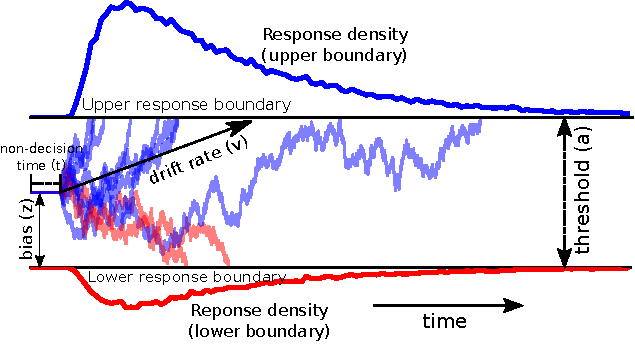
\includegraphics{DDM.pdf}
\caption{Trajectories of multiple drift-processes (blue and red lines, middle panel). Evidence is noisily accumulated over time (x-axis) with average drift-rate \textit{v} until one of two boundaries (separated by threshold \textit{a}) is crossed and a response is initiated. Upper (blue) and lower (red) panels contain density plots over boundary-crossing-times for two possible responses. The flat line in the beginning of the drift-processes denotes the non-decision time \textit{t} where no accumulation happens. The histogram shapes match closely to that observed in reaction time measurements of research participants. Note that HDDM uses a closed-form likelihood function and not actual simulation as depicted here.}\end{figure}

An analytic solution to the resulting probability distribution of
the termination times was provided by \citep{Feller68}:
\begin{gather}
\begin{split}f(x|v, a, z) = \frac{\pi}{a^2} \, \text{exp} \left( -vaz-\frac{v^2\,x}{2} \right) \times \sum_{k=1}^{\infty} k\, \text{exp} \left( -\frac{k^2\pi^2 x}{2a^2} \right) \text{sin}\left(k\pi z\right)\end{split}\notag
\end{gather}
Since the formula contains an infinite sum, HDDM uses an approximation
provided by \citep{NavarroFuss09}.

Subsequently, the DDM was extended to include additional noise parameters capturing inter-trial variability in the drift-rate, the non-decision time and the starting point in order to account for two phenomena observed in decision making tasks, most notably cases where errors are faster or slower than correct responses. Models that take this into account are referred to as the full DDM \citep{RatcliffRouder98}). HDDM uses analytic integration of the likelihood function for variability in drift-rate and numerical integration for variability in non-decision time and bias. More information on the model specifics can be found in \citep{SoferWieckiFrank}.


\subsubsection*{Linear Ballistic Accumulator}
\label{methods:linear-ballistic-accumulator}
The Linear Ballistic Accumulator (LBA) model belongs to the class of
race models \citep{BrownHeathcote08}). Instead of one drift process
and two boundaries, the LBA contains one drift process for each
possible response with a single boundary each. Thus, the LBA can model
decision making when more than two responses are possible. Moreover,
unlike the DDM, the LBA drift process has no intra-trial variance. RT
variability is obtained by including inter-trial variability in the
drift-rate and the starting point distribution. Note that the
simplifying assumption of a noiseless drift-process simplifies the
math significantly leading to a computationally more efficient
likelihood function for this model.

In a simulation study it was shown that the LBA and DDM lead to
similar results as to which parameters are affected by certain
manipulations \citep{DonkinBrownHeathcoteEtAl11}).
\begin{figure}[htbp]
\centering
\capstart

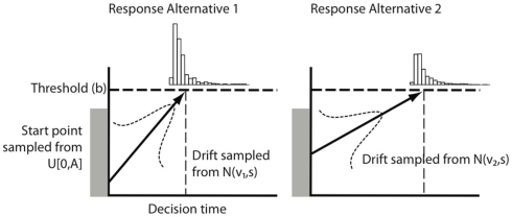
\includegraphics[scale=.6]{lba.png}
\caption{Two linear ballistic accumulators (left and right) with different
noiseless drifts (arrows) sampled from a normal distribution
initiated at different starting points sampled from a uniform
distribution. In this case, the accumulator for response
alternative 1 is more likely to reach the criterion first, and
therefore gets selected more often. Because of this race between
two accumulators towards a common threshold these model are called
race-models. Reproduced from \citep{DonkinBrownHeathcoteEtAl11}.}\end{figure}


\subsection*{Hierarchical Bayesian Estimation}
\label{methods:hierarchical-bayesian-estimation}
Statistics and machine learning have developed efficient and versatile Bayesian methods to solve various inference problems \citep{Poirier06}. More recently, they have seen wider adoption in applied fields such as genetics \citep{StephensBalding09} and psychology \citep{ClemensDeSelenEtAl11}. One reason for this Bayesian revolution is the ability to quantify the certainty one has in a particular estimation of a model parameter. Moreover, hierarchical Bayesian models provide an elegant solution to the problem of estimating parameters of individual subjects and groups of subjects, as outlined above. Under the assumption that participants within each group are similar to each other, but not identical, a hierarchical model can be constructed where individual parameter estimates are constrained by group-level distributions \citep{NilssonRieskampWagenmakers11,ShiffrinLeeKim08}).

Bayesian methods require specification of a generative process in form
of a likelihood function that produced the observed data $x$
given some parameters $\theta$. By specifying our prior beliefs
(which can be informed or non-informed) we can use Bayes formula to
invert the generative model and make inference on the probability of
parameters $\theta$:
\phantomsection\label{methods:bayes}\begin{gather}
\begin{split}P(\theta|x) = \frac{P(x|\theta) \times P(\theta)}{P(x)}\end{split}\notag
\end{gather},
where $P(x|\theta)$ is the likelihood of observing the data (in
this case choices and RTs) given each parameter value and
$P(\theta)$ is the prior probability of the parameters. In most
cases the computation of the denominator is quite complicated and
requires to compute an analytically intractable integral. Sampling
methods like Markov-Chain Monte Carlo (MCMC) \citep{GamermanLopes06}
circumvent this problem by providing a way to produce samples from the
posterior distribution. These methods have been used with great
success in many different scenarios \citep{GelmanCarlinSternEtAl03}
and will be discussed in more detail below.

As noted above, the Bayesian method lends itself naturally to a hierarchical design. In such a design, parameters of a distribution can themselves be expressed as random variables with their own priors. This hierarchical property has a particular benefit to cognitive modeling where data is often scarce: We can construct a hierarchical model that explicitly captures the similarity between individual's parameter values. As above, observed data points of each subject $x_{i,j}$ (where $i = 1, \dots, S_j$ data points per subject and $j = 1, \dots, N$ for $N$ subjects) are distributed according to some likelihood function $f(\theta)$.  We now assume that individual subject parameters $\theta_j$ are normally distributed around a group mean $\mu$ with a specific group standard deviation $\sigma$, resulting in the following generative description:
\begin{gather}
\begin{split}
\theta_j &\sim \mathcal{N}(\mu, \sigma^2) \\
x_{i, j} &\sim f(\theta_j)\end{split}\notag
\end{gather}

\subsection*{Hierarchical Drift-Diffusion Models used in HDDM}
\label{methods:hierarchical-drift-diffusion-models-used-in-hddm}
HDDM includes several hierarchical Bayesian model formulations for the
DDM and LBA. For illustrative purposes we present the graphical model
depiction of a hierarchical DDM model with informative priors and
group only inter-trial variablity parameters. Note, however, that
there is also a model with non-informative priors which the user can opt to use. Nevertheless, we recommend using informative priors as they constrain parameter estimates to be in the range of plausible values based on past literature (see below), which can aid in reducing issues with parameter collinearity, and leads to better recovery of true parameters in simulation studies -- especially with few trials (unpublished results). Specifically, we find that our hierarchical method already provides excellent parameter recovery with as little as 30 trials per condition in a simulation study with 12 subjects.

\begin{figure}[htbp]
\centering
\capstart

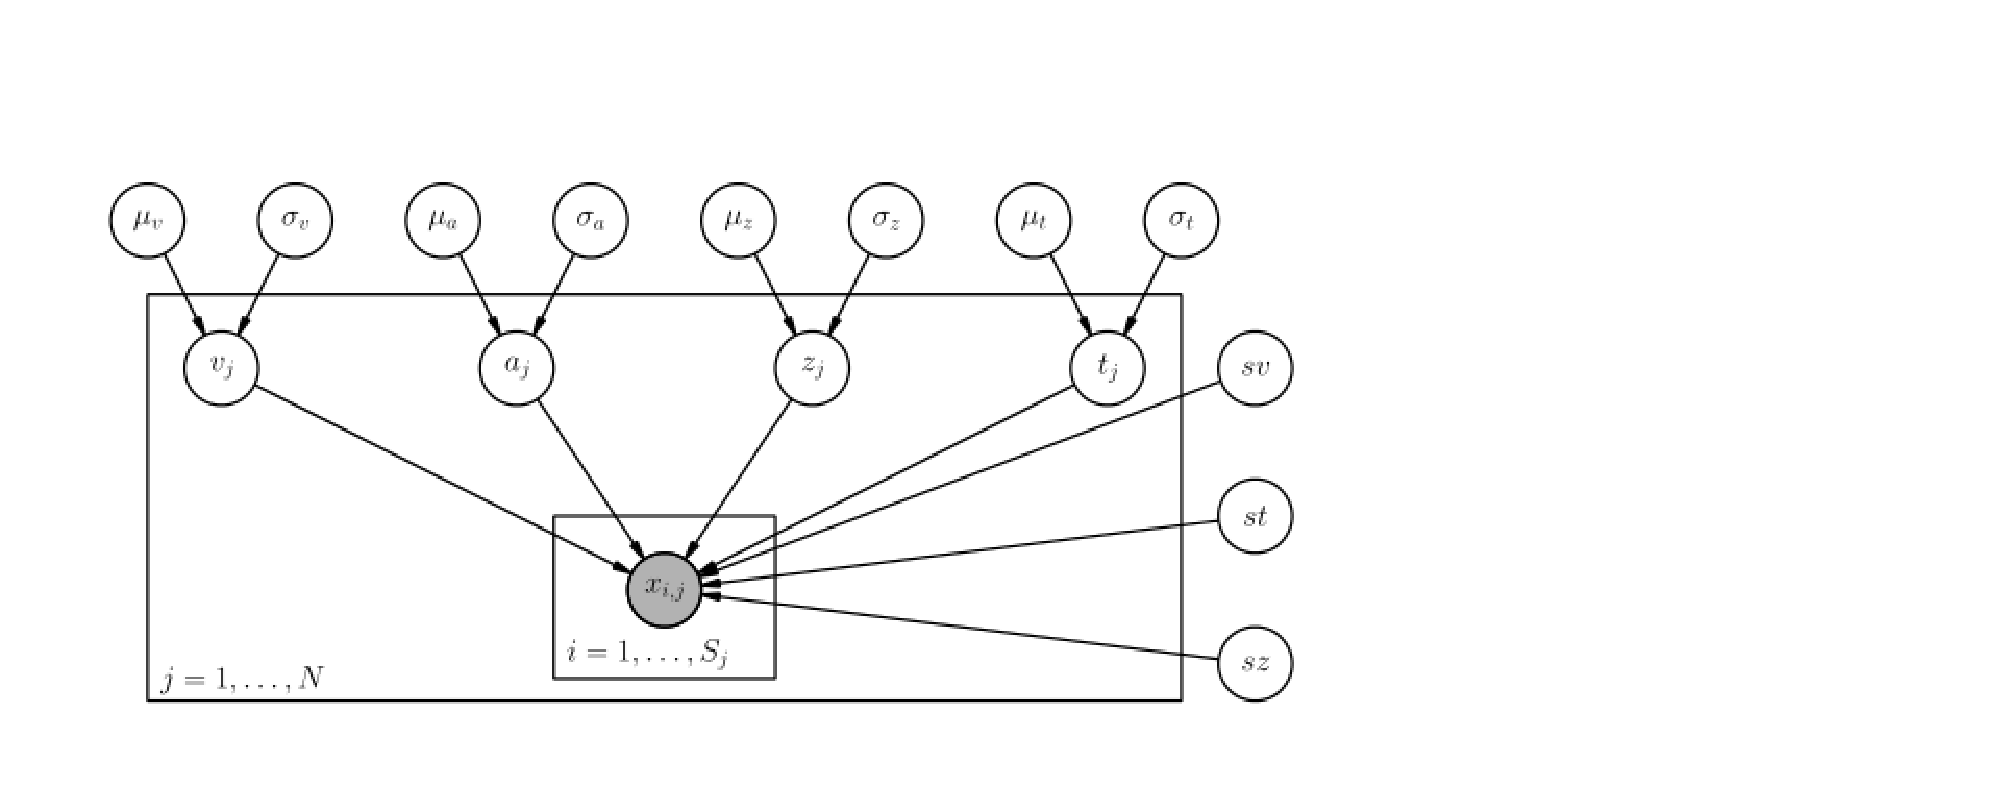
\includegraphics[scale=.7]{graphical_hddm.pdf}
\caption{Basic graphical hierarchical model implemented by HDDM for estimation of the drift-diffusion model. Round nodes represent random variables. Shaded nodes represent observed data. Directed arrows from parents to children visualize that parameters of the child random variable are distributed according to its   parents. Plates denote that multiple random variables with the same   parents and children exist.}\end{figure}

Graphical nodes are distributed as follows:\\
\begin{center}
\begin{tabular}{l|l|l}
$\mu_{a} \sim \mathcal{G}(1.5, 0.75)$ & $\sigma_{a} \sim \mathcal{HN}(0.1)$ & $a_{j} \sim \mathcal{G}(\mu_{a}, \sigma_{a}^2)$ \\
$\mu_{v} \sim \mathcal{N}(2, 3)$ & $\sigma_{v} \sim \mathcal{HN}(2)$ & $v_{j} \sim \mathcal{N}(\mu_{v}, \sigma_{v}^2)$ \\

$\mu_{z} \sim \mathcal{N}(0.5, 0.5)$ & $\sigma_{z} \sim \mathcal{HN}(0.05)$ & $z_{j} \sim \text{invlogit}(\mathcal{N}(\mu_{z}, \sigma_{z}^2))$ \\

$\mu_{t} \sim \mathcal{G}(0.4, 0.2)$ & $\sigma_{t} \sim \mathcal{HN}(1)$ & $t_{j} \sim \mathcal{N}(\mu_{t}, \sigma_{t}^2)$\\

$sv \sim \mathcal{HN}(2)$ & $ster \sim \mathcal{HN}(0.3)$ & $sz \sim \mathcal{B}(1, 3)$
\end{tabular}
\end{center}
and $x_{i, j} \sim F(a_{i}, z_{i}, v_{i}, t_{i}, sv, st, sz)$ where $x_{i, j}$ represents the observed data consisting of
reaction time and choice and $F$ represents the DDM likelihood
function as formulated by \citep{NavarroFuss09}. $\mathcal{N}$
represents a normal distribution parameterized by mean and standard
deviation, $\mathcal{HN}$ represents a half-normal parameterized by
standard-deviation, $\mathcal{G}$ represents a Gamma
distribution parameterized by mean and rate, $\mathcal{B}$
represents a Beta distribution parameterized by $\alpha$ and
$\beta$. Note that in this model we do not attempt to estimate
individual parameters for inter-trial variabilities. The reason is
that the influence of these parameters onto the likelihood is often so
small that very large amounts of data would be required to make
meaningful inference at the individual level.

The informative group mean priors are created to roughly match parameter values reported in the literature and collected by \citep{MatzkeWagenmakers09}. In the below figure we overlayed those empirical values with the prior distribution used for each parameter.
\begin{figure}[htbp]
\centering
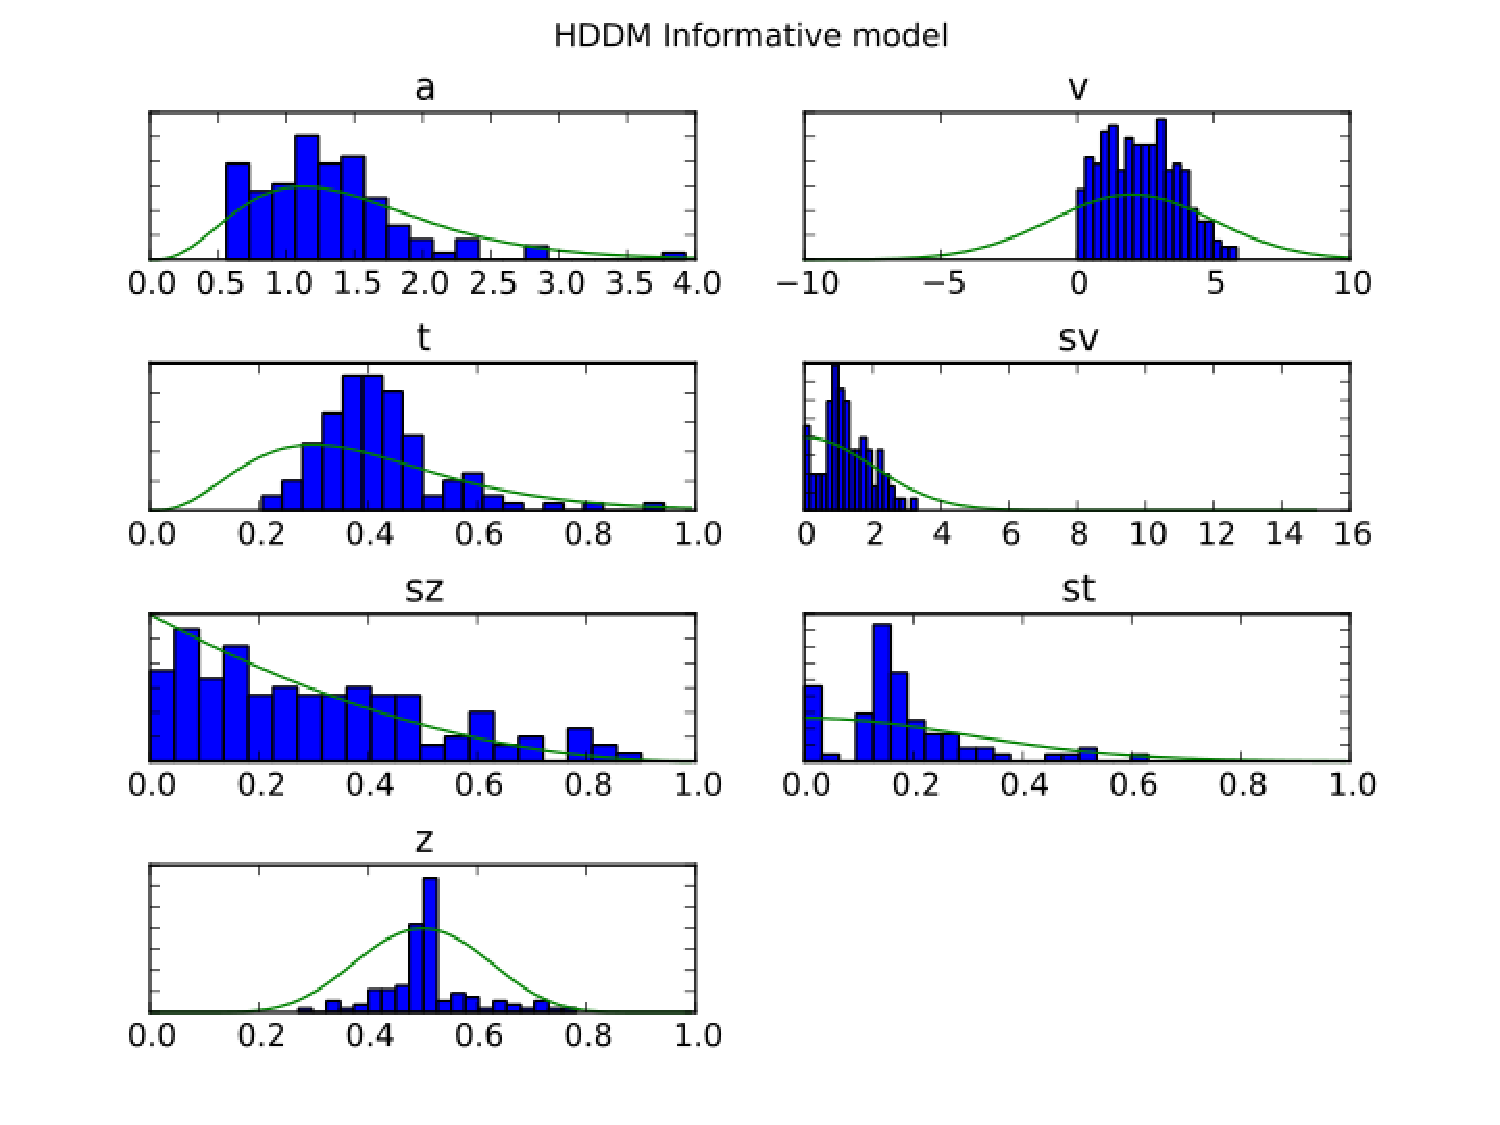
\includegraphics[scale=.5]{hddm_info_priors.pdf}
\caption{Prior distributions.}
\end{figure}

HDDM then uses MCMC to estimate the joint posterior distribution of
all model parameters.

Note that the exact form of the model will be user-dependent; consider as an example a model where separate drift-rates \emph{v} are estimated for two conditions in an experiment: easy and hard. In this case, HDDM will create a hierarchical model with group parameters $\mu_{v_{\text{easy}}}$, $\sigma_{v_{\text{easy}}}$, $\mu_{v_{\text{hard}}}$, $\sigma_{v_{\text{hard}}}$,and individual subject parameters $v_{j_{\text{easy}}}$, and $v_{j_{\text{hard}}}$.

\section*{Results}
\label{demo:index-0}\label{demo:demo}\label{demo:chap-demo}\label{demo::doc}\label{demo:patsy}
In the following we will demonstrate how HDDM can be used to infer different components of the decision making process in a reward-based learning task. While demonstrating core features this is by no means a complete overview of all the functionality in HDDM. For more information, including on how to use HDDM as a command-line utility, online tutorial and a reference manual see \href{http://ski.clps.brown.edu/hddm\_docs}{http://ski.clps.brown.edu/hddm\_docs}.

Python requires modules to be imported before they can be used.
\DUspan{keyword,namespace}{}\DUspan{name,namespace}{}\DUspan{keyword,namespace}{}\DUspan{name,namespace}{}\DUspan{keyword,namespace}{}\DUspan{name,namespace}{}
\begin{Verbatim}[commandchars=\\\{\}]
\PYG{k+kn}{import} \PYG{n+nn}{hddm}
\PYG{k+kn}{import} \PYG{n+nn}{matplotlib.pyplot} \PYG{k+kn}{as} \PYG{n+nn}{plt}
\end{Verbatim}

Matplotlib is a Python module for generating graphics.

\subsection*{Loading data}
\label{demo:loading-data}
It is recommended to store your trial-by-trial reaction time and choice data in a csv (comma-separated-value, see below for exact specifications) file. In this example we will be using data collected in a reward-based decision making experiment in our lab \citep{CavanaghWieckiCohenEtAl11}. In brief, at each trial subjects choose between two symbols. The trials were divided into win-win trials (WW), in which the two symbols were associated with high winning chances; lose-lose trials (LL), in which the symbols were associated with low winning chances, and win-lose trials (WL), which are the easiest because only one symbol was associated with high winning chances. Thus WW and LL decisions together comprise high conflict (HC) trials (although there are other differences between them, we do not focus on those here), whereas WL decisions are low conflict (LC).  The main hypothesis of the study was that high conflict trials induce an increase in the decision threshold, and that the mechanism for this threshold modulation depends on communication between mediofrontal cortex (which exhibits increased activity under conditions of choice uncertainty or conflict) and the subthalamic nucleus (STN) of the basal ganglia (which provides a temporary brake on response selection by increasing the decision threshold). The details of this mechanism are described in other modeling papers \citep[e.g.][]{RatcliffFrank12}. \citet{CavanaghWieckiCohenEtAl11} tested this theory by measuring EEG activity over mid-frontal cortex, focusing on the theta band, given prior associations with conflict, and testing whether trial-to-trial variations in frontal theta were related to adjustments in decision threshold during high conflict trials. They tested the STN component of the theory by administering the same experiment to patients who had deep brain stimulation (DBS) of the STN, which interferes with normal processing.

The first ten lines of the data file look as follows.
\begin{Verbatim}[commandchars=\\\{\}]
\PYG{n}{subj\PYGZus{}idx}\PYG{p}{,}\PYG{n}{stim}\PYG{p}{,}\PYG{n}{rt}\PYG{p}{,}\PYG{n}{response}\PYG{p}{,}\PYG{n}{theta}\PYG{p}{,}\PYG{n}{dbs}\PYG{p}{,}\PYG{n}{conf}
\PYG{l+m+mi}{0}\PYG{p}{,}\PYG{n}{LL}\PYG{p}{,}\PYG{l+m+mf}{1.21}\PYG{p}{,}\PYG{l+m+mf}{1.0}\PYG{p}{,}\PYG{l+m+mf}{0.65}\PYG{p}{,}\PYG{l+m+mi}{1}\PYG{p}{,}\PYG{n}{HC}
\PYG{l+m+mi}{0}\PYG{p}{,}\PYG{n}{WL}\PYG{p}{,}\PYG{l+m+mf}{1.62}\PYG{p}{,}\PYG{l+m+mf}{1.0}\PYG{p}{,}\PYG{o}{\PYGZhy{}}\PYG{l+m+mf}{0.327}\PYG{p}{,}\PYG{l+m+mi}{1}\PYG{p}{,}\PYG{n}{LC}
\PYG{l+m+mi}{0}\PYG{p}{,}\PYG{n}{WW}\PYG{p}{,}\PYG{l+m+mf}{1.03}\PYG{p}{,}\PYG{l+m+mf}{1.0}\PYG{p}{,}\PYG{o}{\PYGZhy{}}\PYG{l+m+mf}{0.480}\PYG{p}{,}\PYG{l+m+mi}{1}\PYG{p}{,}\PYG{n}{HC}
\PYG{l+m+mi}{0}\PYG{p}{,}\PYG{n}{WL}\PYG{p}{,}\PYG{l+m+mf}{2.77}\PYG{p}{,}\PYG{l+m+mf}{1.0}\PYG{p}{,}\PYG{l+m+mf}{1.927}\PYG{p}{,}\PYG{l+m+mi}{1}\PYG{p}{,}\PYG{n}{LC}
\PYG{l+m+mi}{0}\PYG{p}{,}\PYG{n}{WW}\PYG{p}{,}\PYG{l+m+mf}{1.13}\PYG{p}{,}\PYG{l+m+mf}{0.0}\PYG{p}{,}\PYG{o}{\PYGZhy{}}\PYG{l+m+mf}{0.2132}\PYG{p}{,}\PYG{l+m+mi}{1}\PYG{p}{,}\PYG{n}{HC}
\PYG{l+m+mi}{0}\PYG{p}{,}\PYG{n}{WL}\PYG{p}{,}\PYG{l+m+mf}{1.14}\PYG{p}{,}\PYG{l+m+mf}{1.0}\PYG{p}{,}\PYG{o}{\PYGZhy{}}\PYG{l+m+mf}{0.4362}\PYG{p}{,}\PYG{l+m+mi}{1}\PYG{p}{,}\PYG{n}{LC}
\PYG{l+m+mi}{0}\PYG{p}{,}\PYG{n}{LL}\PYG{p}{,}\PYG{l+m+mf}{2.0}\PYG{p}{,}\PYG{l+m+mf}{1.0}\PYG{p}{,}\PYG{o}{\PYGZhy{}}\PYG{l+m+mf}{0.27447}\PYG{p}{,}\PYG{l+m+mi}{1}\PYG{p}{,}\PYG{n}{HC}
\PYG{l+m+mi}{0}\PYG{p}{,}\PYG{n}{WL}\PYG{p}{,}\PYG{l+m+mf}{1.04}\PYG{p}{,}\PYG{l+m+mf}{0.0}\PYG{p}{,}\PYG{l+m+mf}{0.666}\PYG{p}{,}\PYG{l+m+mi}{1}\PYG{p}{,}\PYG{n}{LC}
\PYG{l+m+mi}{0}\PYG{p}{,}\PYG{n}{WW}\PYG{p}{,}\PYG{l+m+mf}{0.856}\PYG{p}{,}\PYG{l+m+mf}{1.0}\PYG{p}{,}\PYG{l+m+mf}{0.1186}\PYG{p}{,}\PYG{l+m+mi}{1}\PYG{p}{,}\PYG{n}{HC}
\end{Verbatim}
The first row represents the column names; each following row corresponds to values associated with a column on an individual trial. While \code{subj\_idx} (unique subject identifier), \code{RT} (reaction time) and \code{response} (binary choice) are required, additional columns can represent experiment specific data. Here, \code{theta} represents theta power as measured by EEG, \code{dbs} whether DBS was turned on or off, \code{stim} which stimulus type was presented and \code{conf} the conflict level of the stimulus (see above).

The \code{hddm.load\_csv()} function can then be used to load this file. \DUspan{name}{}\DUspan{operator}{}\DUspan{name}{}\DUspan{operator}{}\DUspan{name}{}\DUspan{punctuation}{}\DUspan{literal,string}{}\DUspan{punctuation}{}
\begin{Verbatim}[commandchars=\\\{\}]
\PYG{n}{data} \PYG{o}{=} \PYG{n}{hddm}\PYG{o}{.}\PYG{n}{load\PYGZus{}csv}\PYG{p}{(}\PYG{l+s}{\PYGZsq{}}\PYG{l+s}{hddm\PYGZus{}demo.csv}\PYG{l+s}{\PYGZsq{}}\PYG{p}{)}
\end{Verbatim}

To provide the reader with a sense of how RT data is distributed we next plot histograms of each individual's RTs (note the similarity to the DDM density in figure 1). Because there are two possible responses (here we are using accuracy coding where 1 means the more rewarding symbol was chosen, and 0 the less rewarding) we flip error RTs to be
negative.

\DUspan{name}{}\DUspan{operator}{}\DUspan{name}{}\DUspan{operator}{}\DUspan{name}{}\DUspan{operator}{}\DUspan{name}{}\DUspan{punctuation}{}\DUspan{name}{}\DUspan{punctuation}{}\DUspan{name}{}\DUspan{operator}{}\DUspan{name}{}\DUspan{operator}{}\DUspan{name}{}\DUspan{punctuation}{}\DUspan{name}{}\DUspan{operator}{}\DUspan{name}{}\DUspan{operator}{}\DUspan{name}{}\DUspan{punctuation}{}\DUspan{literal,number,integer}{}\DUspan{punctuation}{}\DUspan{name}{}\DUspan{operator}{}\DUspan{literal,string}{}\DUspan{punctuation}{}\DUspan{name}{}\DUspan{operator}{}\DUspan{literal,string}{}\DUspan{punctuation}{}\DUspan{name}{}\DUspan{operator}{}\DUspan{literal,string}{}\DUspan{punctuation}{}\DUspan{keyword}{}\DUspan{name}{}\DUspan{punctuation}{}\DUspan{name}{}\DUspan{operator,word}{}\DUspan{name}{}\DUspan{operator}{}\DUspan{name}{}\DUspan{punctuation}{}\DUspan{literal,string}{}\DUspan{punctuation}{}\DUspan{name}{}\DUspan{operator}{}\DUspan{name}{}\DUspan{punctuation}{}\DUspan{name}{}\DUspan{operator}{}\DUspan{name}{}\DUspan{punctuation}{}\DUspan{name}{}\DUspan{operator}{}\DUspan{literal,number,integer}{}\DUspan{punctuation}{}\DUspan{name}{}\DUspan{operator}{}\DUspan{literal,string}{}\DUspan{punctuation}{}
\begin{Verbatim}[commandchars=\\\{\}]
\PYG{n}{data} \PYG{o}{=} \PYG{n}{hddm}\PYG{o}{.}\PYG{n}{utils}\PYG{o}{.}\PYG{n}{flip\PYGZus{}errors}\PYG{p}{(}\PYG{n}{data}\PYG{p}{)}

\PYG{n}{fig} \PYG{o}{=} \PYG{n}{plt}\PYG{o}{.}\PYG{n}{figure}\PYG{p}{(}\PYG{p}{)}
\PYG{n}{ax} \PYG{o}{=} \PYG{n}{fig}\PYG{o}{.}\PYG{n}{add\PYGZus{}subplot}\PYG{p}{(}\PYG{l+m+mi}{111}\PYG{p}{,} \PYG{n}{xlabel}\PYG{o}{=}\PYG{l+s}{\PYGZsq{}}\PYG{l+s}{RT}\PYG{l+s}{\PYGZsq{}}\PYG{p}{,} \PYG{n}{ylabel}\PYG{o}{=}\PYG{l+s}{\PYGZsq{}}\PYG{l+s}{count}\PYG{l+s}{\PYGZsq{}}\PYG{p}{,} \PYG{n}{title}\PYG{o}{=}\PYG{l+s}{\PYGZsq{}}\PYG{l+s}{RT distributions}\PYG{l+s}{\PYGZsq{}}\PYG{p}{)}
\PYG{k}{for} \PYG{n}{i}\PYG{p}{,} \PYG{n}{subj\PYGZus{}data} \PYG{o+ow}{in} \PYG{n}{data}\PYG{o}{.}\PYG{n}{groupby}\PYG{p}{(}\PYG{l+s}{\PYGZsq{}}\PYG{l+s}{subj\PYGZus{}idx}\PYG{l+s}{\PYGZsq{}}\PYG{p}{)}\PYG{p}{:}
    \PYG{n}{ax}\PYG{o}{.}\PYG{n}{hist}\PYG{p}{(}\PYG{n}{subj\PYGZus{}data}\PYG{o}{.}\PYG{n}{rt}\PYG{p}{,} \PYG{n}{bins}\PYG{o}{=}\PYG{l+m+mi}{20}\PYG{p}{,} \PYG{n}{histtype}\PYG{o}{=}\PYG{l+s}{\PYGZsq{}}\PYG{l+s}{step}\PYG{l+s}{\PYGZsq{}}\PYG{p}{)}
\end{Verbatim}



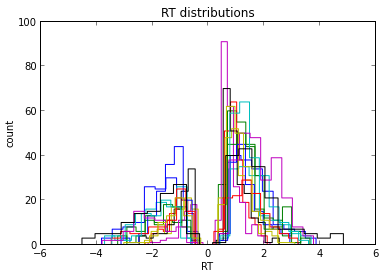
\includegraphics[scale=0.6]{hddm_demo_fig_00.png}


\subsection*{Fitting a hierarchical model}
\label{demo:fitting-a-hierarchical-model}
The previous figure shows that while each individual's RT histogram is different, there is also a lot of similarity. Hierarchical Bayesian modeling allows us to exploit this similarity. The \code{HDDM} class constructs such a hierarchical DDM. To speed up convergence, the starting point is set the maximum a-posterior value (MAP) by calling the \code{HDDM.find\_starting\_values} method. The \code{HDDM.sample()} method then performs Bayesian inference by drawing posterior samples using the MCMC algorithm.
\DUspan{comment}{}\DUspan{comment}{}\DUspan{name}{}\DUspan{operator}{}\DUspan{name}{}\DUspan{operator}{}\DUspan{name}{}\DUspan{punctuation}{}\DUspan{name}{}\DUspan{punctuation}{}\DUspan{comment}{}\DUspan{name}{}\DUspan{operator}{}\DUspan{name}{}\DUspan{punctuation}{}\DUspan{comment}{}\DUspan{name}{}\DUspan{operator}{}\DUspan{name}{}\DUspan{punctuation}{}\DUspan{literal,number,integer}{}\DUspan{punctuation}{}\DUspan{name}{}\DUspan{operator}{}\DUspan{literal,number,integer}{}\DUspan{punctuation}{}
\begin{Verbatim}[commandchars=\\\{\}]
\PYG{c}{\PYGZsh{} Instantiate model object passing it our data (no need to call flip\PYGZus{}errors() before passing it).}
\PYG{c}{\PYGZsh{} This will tailor an individual hierarchical DDM around the dataset.}
\PYG{n}{m} \PYG{o}{=} \PYG{n}{hddm}\PYG{o}{.}\PYG{n}{HDDM}\PYG{p}{(}\PYG{n}{data}\PYG{p}{)}
\PYG{c}{\PYGZsh{} find a good starting point which helps with the convergence.}
\PYG{n}{m}\PYG{o}{.}\PYG{n}{find\PYGZus{}starting\PYGZus{}values}\PYG{p}{(}\PYG{p}{)}
\PYG{c}{\PYGZsh{} start drawing 2000 samples and discarding 20 as burn\PYGZhy{}in}
\PYG{n}{m}\PYG{o}{.}\PYG{n}{sample}\PYG{p}{(}\PYG{l+m+mi}{2000}\PYG{p}{,} \PYG{n}{burn}\PYG{o}{=}\PYG{l+m+mi}{20}\PYG{p}{)}
\end{Verbatim}
We recommend drawing between 2000 and 5000 posterior samples, depending on the convergence. Discarding the first 20-200 samples as burn-in is often enough in our experience. Auto-correlation of the samples can be reduced by adding the \code{thin=n} keyword which only keeps every nth sample, but unless memory is an issue we recommend keeping all samples and increasing the sample size if auto-correlation is high.

Note that it is also possible to fit a non-hierarchical model to an individual subject by setting \code{is\_group\_model=False} in the instantiation of \code{HDDM} or by passing in data which lacks a \code{subj\_idx} column. In this case, HDDM will use the group-mean priors from above for the individual parameters.

It is critical to assess the statistics of our estimated model. The
\code{HDDM.print\_stats()} method outputs a table of summary statistics for each parameters' posterior (note that the output is abridged due to its length).
\DUspan{name}{}\DUspan{operator}{}\DUspan{name}{}\DUspan{operator}{}\DUspan{name}{}\DUspan{punctuation}{}\DUspan{name}{}\DUspan{punctuation}{}\DUspan{name}{}\DUspan{operator}{}\DUspan{name}{}\DUspan{operator}{}\DUspan{name}{}\DUspan{punctuation}{}\DUspan{literal,string}{}\DUspan{punctuation}{}\DUspan{literal,string}{}\DUspan{punctuation}{}\DUspan{literal,string}{}\DUspan{punctuation}{}\DUspan{literal,string}{}\DUspan{punctuation}{}
\begin{Verbatim}[commandchars=\\\{\}]
\PYG{n}{stats} \PYG{o}{=} \PYG{n}{m}\PYG{o}{.}\PYG{n}{gen\PYGZus{}stats}\PYG{p}{(}\PYG{p}{)}
\PYG{n}{stats}\PYG{p}{[}\PYG{n}{stats}\PYG{o}{.}\PYG{n}{index}\PYG{o}{.}\PYG{n}{isin}\PYG{p}{(}\PYG{p}{[}\PYG{l+s}{\PYGZsq{}}\PYG{l+s}{a}\PYG{l+s}{\PYGZsq{}}\PYG{p}{,} \PYG{l+s}{\PYGZsq{}}\PYG{l+s}{a\PYGZus{}var}\PYG{l+s}{\PYGZsq{}}\PYG{p}{,} \PYG{l+s}{\PYGZsq{}}\PYG{l+s}{a\PYGZus{}subj.0}\PYG{l+s}{\PYGZsq{}}\PYG{p}{,} \PYG{l+s}{\PYGZsq{}}\PYG{l+s}{a\PYGZus{}subj.1}\PYG{l+s}{\PYGZsq{}}\PYG{p}{]}\PYG{p}{)}\PYG{p}{]}
\end{Verbatim}

\begin{Verbatim}[commandchars=\\\{\}]
              mean       std      2.5q       25q       50q       75q 97.5q

a         2.058015  0.102570  1.862412  1.988854  2.055198  2.123046 2.261410
a\_var     0.379303  0.089571  0.244837  0.316507  0.367191  0.426531 0.591643
a\_subj.0  2.384066  0.059244  2.274352  2.340795  2.384700  2.423012 2.500647
a\_subj.1  2.127582  0.061901  2.003605  2.086776  2.126963  2.166261 2.254350

\end{Verbatim}

The output contains various summary statistics describing the posterior of each parameter: group mean parameter for
threshold \code{a}, group variability \code{a\_var} and individual subject parameters \code{a\_subj.0}. Other parameters are not shown here but were still estimated.

The inference algorithm, MCMC, requires the chains of the model to have properly converged. While there is no way to guarantee convergence for a finite set of samples in MCMC, there are many heuristics that allow identification of problems of convergence. One main analysis to investigate is the trace, the autocorrelation, and the marginal posterior. These can be plotted using the \code{HDDM.plot\_posteriors()} method. For the sake of brevity we only plot one here. In practice, however, one should examine all of them. \DUspan{name}{}\DUspan{operator}{}\DUspan{name}{}\DUspan{punctuation}{}\DUspan{literal,string}{}\DUspan{punctuation}{}\DUspan{literal,string}{}\DUspan{punctuation}{}\DUspan{literal,string}{}\DUspan{punctuation}{}\DUspan{literal,string}{}\DUspan{punctuation}{}
\begin{Verbatim}[commandchars=\\\{\}]
\PYG{n}{m}\PYG{o}{.}\PYG{n}{plot\PYGZus{}posteriors}\PYG{p}{(}\PYG{p}{[}\PYG{l+s}{\PYGZsq{}}\PYG{l+s}{a', 'a_var}\PYG{l+s}{\PYGZsq{}}{]}\PYG{p}{)}
\end{Verbatim}

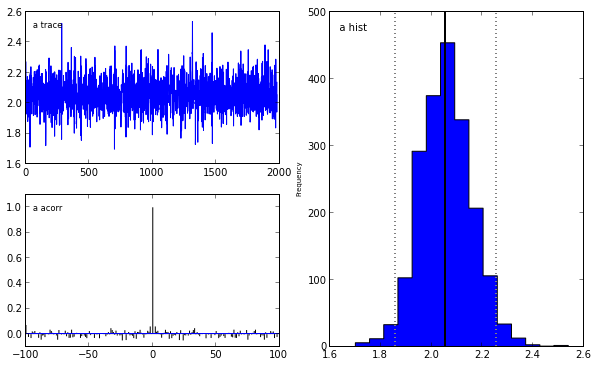
\includegraphics[width=.5\columnwidth]{hddm_demo_fig_01.png}
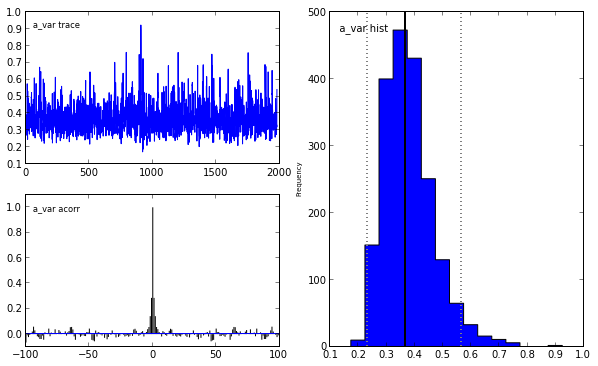
\includegraphics[width=.5\columnwidth]{hddm_demo_fig_02.png}

Problematic patterns in the trace would be drifts or large jumps which are absent here. The autocorrelation should also not be exceedingly high (i.e. well smaller than 50) as is the case here.

The Gelman-Rubin statistic provides a more formal test for convergence
that compares the intra-chain variance to the intra-chain variance of
different runs of the same model. The following code demonstrates how 5 models can be run in a for-loop and stored in a list (here called \code{models}).

\DUspan{name}{}\DUspan{operator}{}\DUspan{punctuation}{}\DUspan{keyword}{}\DUspan{name}{}\DUspan{operator,word}{}\DUspan{name,builtin}{}\DUspan{punctuation}{}\DUspan{literal,number,integer}{}\DUspan{punctuation}{}\DUspan{name}{}\DUspan{operator}{}\DUspan{name}{}\DUspan{operator}{}\DUspan{name}{}\DUspan{punctuation}{}\DUspan{name}{}\DUspan{punctuation}{}\DUspan{name}{}\DUspan{operator}{}\DUspan{name}{}\DUspan{punctuation}{}\DUspan{name}{}\DUspan{operator}{}\DUspan{name}{}\DUspan{punctuation}{}\DUspan{literal,number,integer}{}\DUspan{punctuation}{}\DUspan{name}{}\DUspan{operator}{}\DUspan{literal,number,integer}{}\DUspan{punctuation}{}\DUspan{name}{}\DUspan{operator}{}\DUspan{name}{}\DUspan{punctuation}{}\DUspan{name}{}\DUspan{punctuation}{}\DUspan{name}{}\DUspan{operator}{}\DUspan{name}{}\DUspan{operator}{}\DUspan{name}{}\DUspan{punctuation}{}\DUspan{name}{}\DUspan{punctuation}{}
\begin{Verbatim}[commandchars=\\\{\}]
\PYG{n}{models} \PYG{o}{=} \PYG{p}{[}\PYG{p}{]}
\PYG{k}{for} \PYG{n}{i} \PYG{o+ow}{in} \PYG{n+nb}{range}\PYG{p}{(}\PYG{l+m+mi}{5}\PYG{p}{)}\PYG{p}{:}
    \PYG{n}{m} \PYG{o}{=} \PYG{n}{hddm}\PYG{o}{.}\PYG{n}{HDDM}\PYG{p}{(}\PYG{n}{data}\PYG{p}{)}
    \PYG{n}{m}\PYG{o}{.}\PYG{n}{find\PYGZus{}starting\PYGZus{}values}\PYG{p}{(}\PYG{p}{)}
    \PYG{n}{m}\PYG{o}{.}\PYG{n}{sample}\PYG{p}{(}\PYG{l+m+mi}{5000}\PYG{p}{,} \PYG{n}{burn}\PYG{o}{=}\PYG{l+m+mi}{20}\PYG{p}{)}
    \PYG{n}{models}\PYG{o}{.}\PYG{n}{append}\PYG{p}{(}\PYG{n}{m}\PYG{p}{)}

\PYG{n}{hddm}\PYG{o}{.}\PYG{n}{analyze}\PYG{o}{.}\PYG{n}{gelman\PYGZus{}rubin}\PYG{p}{(}\PYG{n}{models}\PYG{p}{)}
\end{Verbatim}

Which produces the following output (abridged to preserve space):
\begin{Verbatim}[commandchars=\\\{\}]
\PYG{p}{\PYGZob{}}\PYG{l+s}{\PYGZsq{}}\PYG{l+s}{a}\PYG{l+s}{\PYGZsq{}}\PYG{p}{:} \PYG{l+m+mf}{1.000}\PYG{p}{,}
 \PYG{l+s}{\PYGZsq{}}\PYG{l+s}{a\PYGZus{}std}\PYG{l+s}{\PYGZsq{}}\PYG{p}{:} \PYG{l+m+mf}{1.001}\PYG{p}{,}
 \PYG{l+s}{\PYGZsq{}}\PYG{l+s}{t}\PYG{l+s}{\PYGZsq{}}\PYG{p}{:} \PYG{l+m+mf}{1.000}\PYG{p}{\PYGZcb{}}
\end{Verbatim}

Values should be close to 1 and not larger than 1.02 which would indicate convergence problems.

To test whether the different conflict conditions affect drift-rate we create a new model which estimates separate drift-rate \code{v} for the three conflict conditions. HDDM supports splitting by condition via the \code{depends\_on} keyword argument supplied to the \code{HDDM} class. This argument expects a Python \code{dict} which maps the parameter to be split to the column name containing the conditions we want to split by. This way of defining parameters to be split by condition is directly inspired by the fast-dm toolbox \citep{VossVoss07}. \DUspan{name}{}\DUspan{operator}{}\DUspan{name}{}\DUspan{operator}{}\DUspan{name}{}\DUspan{punctuation}{}\DUspan{name}{}\DUspan{punctuation}{}\DUspan{name}{}\DUspan{operator}{}\DUspan{punctuation}{}\DUspan{literal,string}{}\DUspan{punctuation}{}\DUspan{literal,string}{}\DUspan{punctuation}{}\DUspan{name}{}\DUspan{operator}{}\DUspan{name}{}\DUspan{punctuation}{}\DUspan{name}{}\DUspan{operator}{}\DUspan{name}{}\DUspan{punctuation}{}\DUspan{literal,number,integer}{}\DUspan{punctuation}{}\DUspan{name}{}\DUspan{operator}{}\DUspan{literal,number,integer}{}\DUspan{punctuation}{}
\begin{Verbatim}[commandchars=\\\{\}]
\PYG{n}{m\PYGZus{}stim} \PYG{o}{=} \PYG{n}{hddm}\PYG{o}{.}\PYG{n}{HDDM}\PYG{p}{(}\PYG{n}{data}\PYG{p}{,} \PYG{n}{depends\PYGZus{}on}\PYG{o}{=}\PYG{p}{\PYGZob{}}\PYG{l+s}{\PYGZsq{}}\PYG{l+s}{v}\PYG{l+s}{\PYGZsq{}}\PYG{p}{:} \PYG{l+s}{\PYGZsq{}}\PYG{l+s}{stim}\PYG{l+s}{\PYGZsq{}}\PYG{p}{\PYGZcb{}}\PYG{p}{)}
\PYG{n}{m\PYGZus{}stim}\PYG{o}{.}\PYG{n}{find\PYGZus{}starting\PYGZus{}values}\PYG{p}{(}\PYG{p}{)}
\PYG{n}{m\PYGZus{}stim}\PYG{o}{.}\PYG{n}{sample}\PYG{p}{(}\PYG{l+m+mi}{2000}\PYG{p}{,} \PYG{n}{burn}\PYG{o}{=}\PYG{l+m+mi}{20}\PYG{p}{)}
\end{Verbatim}

Note that while here every subject was tested on each condition this is not a requirement. The \code{depends\_on} keyword can also be used to test between-group differences. For example, if we collected data where one group received a drug and the other one a placebo we would include a column in the data labeled 'drug' that contained 'drug' or 'placebo' for each subject. In our model specification we could test the hypothesis that the drug affects threshold by specifying \code{depends\_on=\{'a': 'drug'\}}.

We next turn to comparing the posterior for the different drift-rate conditions. To plot the different traces we need to access the underlying node object. These are stored inside the \code{nodes\_db} attribute which is a table (specifically, a \code{Pandas} \code{DataFrame}) containing each model parameter as rows (e.g. \code{v(WW)}) and the correspond information about that parameter columns. The \code{node} column used here represents the \code{PyMC} node object. Multiple assignment is then used to assign the 3 drift-rate nodes to separate variables. \DUspan{name}{}\DUspan{punctuation}{}\DUspan{name}{}\DUspan{punctuation}{}\DUspan{name}{}\DUspan{operator}{}\DUspan{name}{}\DUspan{operator}{}\DUspan{name}{}\DUspan{operator}{}\DUspan{name}{}\DUspan{punctuation}{}\DUspan{literal,string}{}\DUspan{punctuation}{}\DUspan{literal,string}{}\DUspan{punctuation}{}\DUspan{literal,string}{}\DUspan{punctuation}{}\DUspan{name}{}\DUspan{operator}{}\DUspan{name}{}\DUspan{operator}{}\DUspan{name}{}\DUspan{punctuation}{}\DUspan{name}{}\DUspan{punctuation}{}\DUspan{name}{}\DUspan{punctuation}{}\DUspan{name}{}\DUspan{punctuation}{}
\begin{Verbatim}[commandchars=\\\{\}]
\PYG{n}{v\PYGZus{}WW}\PYG{p}{,} \PYG{n}{v\PYGZus{}LL}\PYG{p}{,} \PYG{n}{v\PYGZus{}WL} \PYG{o}{=} \PYG{n}{m\PYGZus{}stim}\PYG{o}{.}\PYG{n}{nodes\PYGZus{}db}\PYG{o}{.}\PYG{n}{node}\PYG{p}{[}\PYG{p}{[}\PYG{l+s}{\PYGZsq{}}\PYG{l+s}{v(WW)}\PYG{l+s}{\PYGZsq{}}\PYG{p}{,} \PYG{l+s}{\PYGZsq{}}\PYG{l+s}{v(LL)}\PYG{l+s}{\PYGZsq{}}\PYG{p}{,} \PYG{l+s}{\PYGZsq{}}\PYG{l+s}{v(WL)}\PYG{l+s}{\PYGZsq{}}\PYG{p}{]}\PYG{p}{]}
\PYG{n}{hddm}\PYG{o}{.}\PYG{n}{analyze}\PYG{o}{.}\PYG{n}{plot\PYGZus{}posterior\PYGZus{}nodes}\PYG{p}{(}\PYG{p}{[}\PYG{n}{v\PYGZus{}WW}\PYG{p}{,} \PYG{n}{v\PYGZus{}LL}\PYG{p}{,} \PYG{n}{v\PYGZus{}WL}\PYG{p}{]}\PYG{p}{)}
\end{Verbatim}

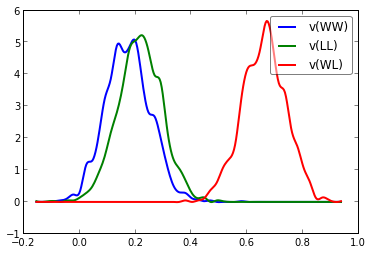
\includegraphics[scale=.7]{hddm_demo_fig_06.png}
Based on the above figure we might reason that the \code{WL} condition drift-rate is substantially greater than that for the other two conditions, which are fairly similar to each other.

One benefit of estimating the model in a Bayesian framework is that we can do significance testing directly on the posterior rather than relying on frequentist statistics \citep{Lindley65} (see also \citet{Kruschke10} for many examples of the advantages of this approach). For example, we might be interested in whether the drift-rate for \code{WW} is larger than that for \code{LL}, or whether drift-rate for \code{LL} is larger than \code{WL}. The below code computes the proportion of the posteriors in which the drift rate for one condition is greater than the other. It can be seen that the posteriors for \code{LL} do not overlap at all for \code{WL}, and thus the probability that \code{LL} is greater than \code{WL} should be near zero. \DUspan{keyword}{}\DUspan{literal,string}{}\DUspan{punctuation}{}\DUspan{punctuation}{}\DUspan{name}{}\DUspan{operator}{}\DUspan{name}{}\DUspan{punctuation}{}\DUspan{operator}{}\DUspan{name}{}\DUspan{operator}{}\DUspan{name}{}\DUspan{punctuation}{}\DUspan{operator}{}\DUspan{name}{}\DUspan{punctuation}{}\DUspan{keyword}{}\DUspan{literal,string}{}\DUspan{punctuation}{}\DUspan{punctuation}{}\DUspan{name}{}\DUspan{operator}{}\DUspan{name}{}\DUspan{punctuation}{}\DUspan{operator}{}\DUspan{name}{}\DUspan{operator}{}\DUspan{name}{}\DUspan{punctuation}{}\DUspan{operator}{}\DUspan{name}{}\DUspan{punctuation}{}
\begin{Verbatim}[commandchars=\\\{\}]
\PYG{k}{print} \PYG{l+s}{\PYGZdq{}}\PYG{l+s}{P(WW \PYGZgt{} LL) = }\PYG{l+s}{\PYGZdq{}}\PYG{p}{,} \PYG{p}{(}\PYG{n}{v\PYGZus{}WW}\PYG{o}{.}\PYG{n}{trace}\PYG{p}{(}\PYG{p}{)} \PYG{o}{\PYGZgt{}} \PYG{n}{v\PYGZus{}LL}\PYG{o}{.}\PYG{n}{trace}\PYG{p}{(}\PYG{p}{)}\PYG{p}{)}\PYG{o}{.}\PYG{n}{mean}\PYG{p}{(}\PYG{p}{)}
\PYG{k}{print} \PYG{l+s}{\PYGZdq{}}\PYG{l+s}{P(LL \PYGZgt{} WL) = }\PYG{l+s}{\PYGZdq{}}\PYG{p}{,} \PYG{p}{(}\PYG{n}{v\PYGZus{}LL}\PYG{o}{.}\PYG{n}{trace}\PYG{p}{(}\PYG{p}{)} \PYG{o}{\PYGZgt{}} \PYG{n}{v\PYGZus{}WL}\PYG{o}{.}\PYG{n}{trace}\PYG{p}{(}\PYG{p}{)}\PYG{p}{)}\PYG{o}{.}\PYG{n}{mean}\PYG{p}{(}\PYG{p}{)}
\end{Verbatim}

\begin{Verbatim}[commandchars=\\\{\}]
\PYG{n}{P}\PYG{p}{(}\PYG{n}{WW} \PYG{o}{\PYGZgt{}} \PYG{n}{LL}\PYG{p}{)} \PYG{o}{=}  \PYG{l+m+mf}{0.34696969697}
\PYG{n}{P}\PYG{p}{(}\PYG{n}{LL} \PYG{o}{\PYGZgt{}} \PYG{n}{WL}\PYG{p}{)} \PYG{o}{=}  \PYG{l+m+mf}{0.0}
\end{Verbatim}

In addition to computing the overlap of the posterior distributions we can compare two models using the deviance information criterion (DIC; lower is better). Note that the DIC measures the fit of the model to the data, penalizing for complexity in the addition of degrees of freedom (the model with three drift rates has more dF than the model with one). The DIC is known to be somewhat biased in selecting the model with greater complexity, although alternative forms exist which improve this issue \citep[see][]{Plummer08}. Nevertheless, DIC can be a useful metric with this caveat in mind. One suggested approach is to generate simulated data from alternative models and use DIC to determine whether it properly selects the correct model given the same task contingencies. This exercise can help determine whether to rely on DIC, and also to provide an expected quantitative difference in DIC scores between models if one of them was correct, as a benchmark to compare DIC differences for fits to real data.
 \DUspan{keyword}{}\DUspan{literal,string}{}\DUspan{literal,string,interpol}{}\DUspan{literal,string}{}\DUspan{operator}{}\DUspan{name}{}\DUspan{operator}{}\DUspan{name}{}\DUspan{keyword}{}\DUspan{literal,string}{}\DUspan{literal,string,interpol}{}\DUspan{literal,string}{}\DUspan{operator}{}\DUspan{name}{}\DUspan{operator}{}\DUspan{name}{}
\begin{Verbatim}[commandchars=\\\{\}]
\PYG{k}{print} \PYG{l+s}{\PYGZdq{}}\PYG{l+s}{Lumped model DIC: }\PYG{l+s+si}{\PYGZpc{}f}\PYG{l+s}{\PYGZdq{}} \PYG{o}{\PYGZpc{}} \PYG{n}{m}\PYG{o}{.}\PYG{n}{dic}
\PYG{k}{print} \PYG{l+s}{\PYGZdq{}}\PYG{l+s}{Stimulus model DIC: }\PYG{l+s+si}{\PYGZpc{}f}\PYG{l+s}{\PYGZdq{}} \PYG{o}{\PYGZpc{}} \PYG{n}{m\PYGZus{}stim}\PYG{o}{.}\PYG{n}{dic}
\end{Verbatim}

\begin{Verbatim}[commandchars=\\\{\}]
Lumped model DIC: 10960.570932
Stimulus model DIC: 10775.615192
\end{Verbatim}

Based on the lower DIC score for the model allowing drift-rate to vary by stimulus condition we might conclude that it provides better fit than the model which forces the drift-rates to be equal, despite the increased complexity.

\subsection*{Within-subject effects}
\label{demo:within-subject-effects}
Note that while the \code{m\_stim} model we created above estimates different drift-rates \code{v} for each subject, it implicitly assumes that the different conditions are completely independent:  each drift rate was sampled from a separate group prior. However, there may be individual differences in overall performance, and if so it is reasonable to assume that someone who would be better at \code{WL} would also be better at \code{LL}. To model this intuition we can use a within-subject model where an intercept is used to capture overall performance in the \code{WL} condition as a baseline, and then the other \code{LL} and \code{WW} conditions are expressed relative to \code{WL}. (Perhaps every subject has a higher drift in \code{WL} than \code{LL} but there is huge variance in their overall drift rates. In this scenario, the earlier model would not have the power to detect the effect of condition on this within subject effect, because there would be large posterior variance in all of the drift rates, which would then overlap with each other.  In contrast, the within-subject model would estimate large variance in the intercept but still allow the model to infer a non-zero effect of condition with high precision).

The \code{HDDMRegressor} class allows individual parameters to be described by a linear model specification. As can be seen below, by specifying a linear model that uses categorical dummy-coding we can estimate within-subject effects. In addition to the data argument, \code{HDDMRegressor} expects a linear model descriptor string to be provided. This descriptor contains the \code{outcome} variable that should be replaced with the output of the linear model -- in this case \code{v}. The \code{C()} specifies that the \code{stim} column contains categorical data and will result in \code{WL}, \code{LL}, and \code{WW} being dummy coded. The \code{Treatment} argument encodes which condition should be used as the intercept. The two other conditions -- \code{LL} and \code{WW} -- will then be expressed \textit{relative} to \code{WL}. Internally, \code{HDDMRegressor} uses the \code{Patsy} module to construct a design matrix from the linear model descriptor, see \href{https://patsy.readthedocs.org/en/latest/}{https://patsy.readthedocs.org/en/latest/} for more details. \DUspan{name}{}\DUspan{operator}{}\DUspan{name}{}\DUspan{operator}{}\DUspan{name}{}\DUspan{punctuation}{}\DUspan{name}{}\DUspan{punctuation}{}\DUspan{literal,string}{}\DUspan{punctuation}{}
\begin{Verbatim}[commandchars=\\\{\}]
\PYG{n}{m\PYGZus{}within\PYGZus{}subj} \PYG{o}{=} \PYG{n}{hddm}\PYG{o}{.}\PYG{n}{HDDMRegressor}\PYG{p}{(}\PYG{n}{data}\PYG{p}{,} \PYG{l+s}{\PYGZdq{}}\PYG{l+s}{v \PYGZti{} C(stim, Treatment(}\PYG{l+s}{\PYGZsq{}}\PYG{l+s}{WL}\PYG{l+s}{\PYGZsq{}}\PYG{l+s}{))}\PYG{l+s}{\PYGZdq{}}\PYG{p}{)}
\end{Verbatim}

Which outputs the newly created covariates which will be used in the regression:
\begin{Verbatim}[commandchars=\\\{\}]
Adding these covariates:
['v\_Intercept', "v\_C(stim, Treatment('WL'))[T.LL]", "v\_C(stim, Treatment('WL'))[T.WW]"]
\end{Verbatim}
As alluded to above, \code{WL} will be used as the intercept. \code{v\_C(stim, Treatment('WL'))[T.LL]} and \code{v\_C(stim, Treatment('WL'))[T.WW]} are new parameters that will be estimated relative to the intercept.

To estimate the model we again draw samples from the posterior:
\DUspan{name}{}\DUspan{operator}{}\DUspan{name}{}\DUspan{punctuation}{}\DUspan{literal,number,integer}{}\DUspan{punctuation}{}\DUspan{name}{}\DUspan{operator}{}\DUspan{literal,number,integer}{}\DUspan{punctuation}{}
\begin{Verbatim}[commandchars=\\\{\}]
\PYG{n}{m\PYGZus{}within\PYGZus{}subj}\PYG{o}{.}\PYG{n}{sample}\PYG{p}{(}\PYG{l+m+mi}{5000}\PYG{p}{,} \PYG{n}{burn}\PYG{o}{=}\PYG{l+m+mi}{200}\PYG{p}{)}
\end{Verbatim}
\DUspan{name}{}\DUspan{punctuation}{}\DUspan{name}{}\DUspan{punctuation}{}\DUspan{name}{}\DUspan{operator}{}\DUspan{name}{}\DUspan{operator}{}\DUspan{name}{}\DUspan{operator}{}\DUspan{name}{}\DUspan{punctuation}{}\DUspan{literal,string}{}\DUspan{punctuation}{}\DUspan{literal,string}{}\DUspan{punctuation}{}\DUspan{literal,string}{}\DUspan{punctuation}{}\DUspan{name}{}\DUspan{operator}{}\DUspan{name}{}\DUspan{operator}{}\DUspan{name}{}\DUspan{punctuation}{}\DUspan{name}{}\DUspan{punctuation}{}\DUspan{name}{}\DUspan{punctuation}{}\DUspan{name}{}\DUspan{punctuation}{}

To examine the marginal posteriors of our individual regressors we can again plot them:
\begin{Verbatim}[commandchars=\\\{\}]
\PYG{n}{v\PYGZus{}WL}\PYG{p}{,} \PYG{n}{v\PYGZus{}LL}\PYG{p}{,} \PYG{n}{v\PYGZus{}WW} \PYG{o}{=} \PYG{n}{m\PYGZus{}within\PYGZus{}subj}\PYG{o}{.}\PYG{n}{nodes\PYGZus{}db}\PYG{o}{.}\PYG{n}{node}\PYG{p}{[}\PYG{p}{[}\PYG{l+s}{\PYGZdq{}}\PYG{l+s}{v\PYGZus{}Intercept}\PYG{l+s}{\PYGZdq{}}\PYG{p}{,}
                                                \PYG{l+s}{\PYGZdq{}}\PYG{l+s}{v\PYGZus{}C(stim, Treatment(}\PYG{l+s}{\PYGZsq{}}\PYG{l+s}{WL}\PYG{l+s}{\PYGZsq{}}\PYG{l+s}{))[T.LL]}\PYG{l+s}{\PYGZdq{}}\PYG{p}{,}
                                                \PYG{l+s}{\PYGZdq{}}\PYG{l+s}{v\PYGZus{}C(stim, Treatment(}\PYG{l+s}{\PYGZsq{}}\PYG{l+s}{WL}\PYG{l+s}{\PYGZsq{}}\PYG{l+s}{))[T.WW]}\PYG{l+s}{\PYGZdq{}}\PYG{p}{]}\PYG{p}{]}
\PYG{n}{hddm}\PYG{o}{.}\PYG{n}{analyze}\PYG{o}{.}\PYG{n}{plot\PYGZus{}posterior\PYGZus{}nodes}\PYG{p}{(}\PYG{p}{[}\PYG{n}{v\PYGZus{}WL}\PYG{p}{,} \PYG{n}{v\PYGZus{}LL}\PYG{p}{,} \PYG{n}{v\PYGZus{}WW}\PYG{p}{]}\PYG{p}{)}
\end{Verbatim}

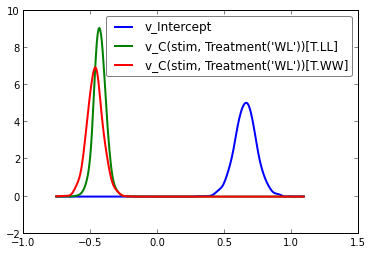
\includegraphics[scale=.7]{hddm_demo_fig_07.png}

Note that in the above plot \code{LL} and \code{WW} are expressed relative to the \code{WL} condition (i.e. \code{v\_Intercept}). Thus, while the overall drift rate intercept, here applying to the \code{WL} condition, is positive (mode value roughly 0.7), the relative within subject effects of condition (\code{WW} and \code{LL}) are negative and do not overlap with zero -- suggesting a significant effect of this condition on drift-rate.

\subsection*{Fitting regression models}
\label{demo:fitting-regression-models}
As mentioned above, cognitive neuroscience has embraced the DDM as it enables to link psychological processes to cognitive brain measures. The \citet{CavanaghWieckiCohenEtAl11} study provides a useful illustration of the functionaility. EEG recordings provided a trial-ty-trial measure of brain activity (frontal theta), and it was found that this activity correlated with increases in decision threshold in high conflict trials. Note that the data set and results exhibit more features than we consider here for the time being (specifically the manipulation of deep brain stimulation), but for illustrative purposes, we replicate here the main theta-threshold relationship in a model restricted to participants without brain stimulation. For more information, see \citet{CavanaghWieckiCohenEtAl11} \DUspan{name}{}\DUspan{operator}{}\DUspan{name}{}\DUspan{operator}{}\DUspan{name}{}\DUspan{punctuation}{}\DUspan{name}{}\DUspan{punctuation}{}\DUspan{name}{}\DUspan{operator}{}\DUspan{name}{}\DUspan{operator}{}\DUspan{literal,number,integer}{}\DUspan{punctuation}{}\DUspan{literal,string}{}\DUspan{punctuation}{}\DUspan{name}{}\DUspan{operator}{}\DUspan{punctuation}{}\DUspan{literal,string}{}\DUspan{punctuation}{}\DUspan{literal,string}{}\DUspan{punctuation}{}\DUspan{name}{}\DUspan{operator}{}\DUspan{name,builtin,pseudo}{}\DUspan{punctuation}{}
\begin{Verbatim}[commandchars=\\\{\}]
\PYG{n}{m\PYGZus{}reg} \PYG{o}{=} \PYG{n}{hddm}\PYG{o}{.}\PYG{n}{HDDMRegressor}\PYG{p}{(}\PYG{n}{data}\PYG{p}{[}\PYG{n}{data}\PYG{o}{.}\PYG{n}{dbs} \PYG{o}{==} \PYG{l+m+mi}{0}\PYG{p}{]}\PYG{p}{,}
                           \PYG{l+s}{\PYGZdq{}}\PYG{l+s}{a \PYGZti{} theta:C(conf, Treatment(}\PYG{l+s}{\PYGZsq{}}\PYG{l+s}{LC}\PYG{l+s}{\PYGZsq{}}\PYG{l+s}{))}\PYG{l+s}{\PYGZdq{}}\PYG{p}{,}
                           \PYG{n}{depends\PYGZus{}on}\PYG{o}{=}\PYG{p}{\PYGZob{}}\PYG{l+s}{\PYGZsq{}}\PYG{l+s}{v}\PYG{l+s}{\PYGZsq{}}\PYG{p}{:} \PYG{l+s}{\PYGZsq{}}\PYG{l+s}{stim}\PYG{l+s}{\PYGZsq{}}\PYG{p}{\PYGZcb{}}\PYG{p}{)}
\end{Verbatim}

Which produces the following output:
\begin{Verbatim}[commandchars=\\\{\}]
Adding these covariates:
['a\_Intercept', "a\_theta:C(conf, Treatment('LC'))[HC]", "a\_theta:C(conf, Treatment('LC'))[LC]"]
\end{Verbatim}

Instead of estimating one static threshold per subject across trials, this model assumes the threshold to vary on each trial according to the linear model specified above (as a function of their measured theta activity). \citet{CavanaghWieckiCohenEtAl11} illustrates that this brain/behavior relationship differs as a function of whether patients are on or off STN deep brain stimulation, as hypothesized by the model that STN is responsible for increasing the decision threshold when cortical theta rises).

As noted above, this experiment also tested patients on deep brain stimulation (DBS). The below figure shows the regression coefficient of theta on threshold when the above model is estimated in the DBS off condition (in blue) and the DBS on condition (in green; code to estimate not shown). As can be seen, the influence of theta on threshold reverses. This exercise thus shows that HDDM can be used both to assess the influence of trial-by-trial brain measures on DDM parameters, but also how parameters vary when brain state is manipulated.

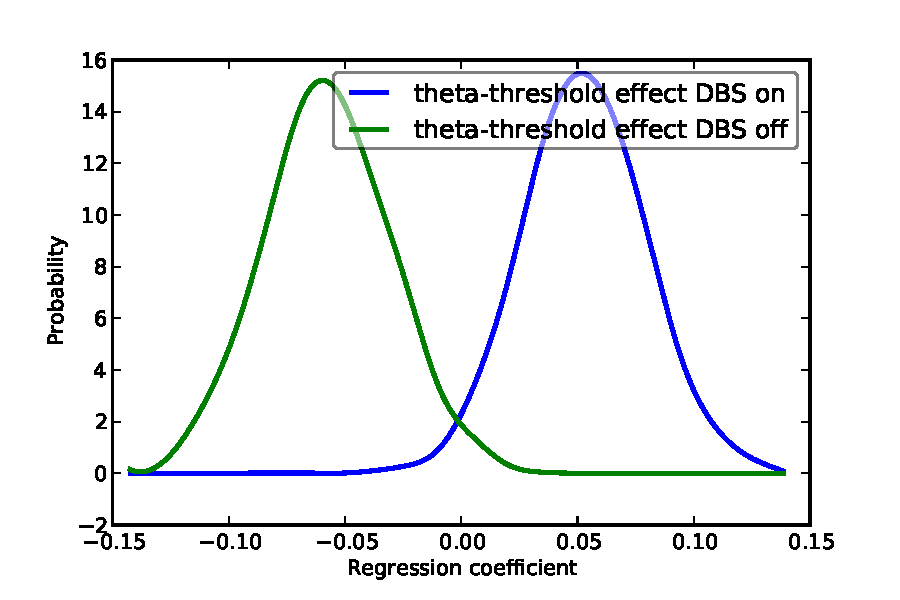
\includegraphics[scale=0.6]{theta_threshold_on_off.pdf}

\subsection*{Dealing with outliers}
\label{demo:dealing-with-outliers}
It is common to have outliers in any data set and RT data are no exception. Outliers present a serious challenge to likelihood-based approaches, as used in HDDM. Consider the possibility that 5\% of trials are not generated by the DDM process, but by some other process (e.g.  due to an attentional lapse). The observed data in those trials may be very unlikely given the best DDM parameters that fit 95\% of the data.  In the extreme case, the likelihood of a single trial may be zero (e.g.  if subjects respond very quickly, faster than the non-decision time \code{t} parameter that would fit the rest of the data). Thus this single outlier would force the DDM parameters to adjust substantially. To illustrate the effect of this we will generate data with outliers, but fit a standard DDM model without taking outliers into account. \DUspan{name}{}\DUspan{punctuation}{}\DUspan{name}{}\DUspan{operator}{}\DUspan{name}{}\DUspan{operator}{}\DUspan{name}{}\DUspan{operator}{}\DUspan{name}{}\DUspan{punctuation}{}\DUspan{name}{}\DUspan{operator}{}\DUspan{punctuation}{}\DUspan{literal,string}{}\DUspan{punctuation}{}\DUspan{literal,number,integer}{}\DUspan{punctuation}{}\DUspan{literal,string}{}\DUspan{punctuation}{}\DUspan{operator}{}\DUspan{literal,number,integer}{}\DUspan{punctuation}{}\DUspan{literal,string}{}\DUspan{punctuation}{}\DUspan{operator}{}\DUspan{literal,number,integer}{}\DUspan{punctuation}{}\DUspan{name}{}\DUspan{operator}{}\DUspan{literal,number,integer}{}\DUspan{punctuation}{}\DUspan{name}{}\DUspan{operator}{}\DUspan{literal,number,integer}{}\DUspan{punctuation}{}
\begin{Verbatim}[commandchars=\\\{\}]
\PYG{n}{outlier\PYGZus{}data}\PYG{p}{,} \PYG{n}{params} \PYG{o}{=} \PYG{n}{hddm}\PYG{o}{.}\PYG{n}{generate}\PYG{o}{.}\PYG{n}{gen\PYGZus{}rand\PYGZus{}data}\PYG{p}{(}\PYG{n}{params}\PYG{o}{=}\PYG{p}{\PYGZob{}}\PYG{l+s}{\PYGZsq{}}\PYG{l+s}{a}\PYG{l+s}{\PYGZsq{}}\PYG{p}{:} \PYG{l+m+mi}{2}\PYG{p}{,} \PYG{l+s}{\PYGZsq{}}\PYG{l+s}{t}\PYG{l+s}{\PYGZsq{}}\PYG{p}{:} \PYG{o}{.}\PYG{l+m+mi}{4}\PYG{p}{,} \PYG{l+s}{\PYGZsq{}}\PYG{l+s}{v}\PYG{l+s}{\PYGZsq{}}\PYG{p}{:} \PYG{o}{.}\PYG{l+m+mi}{5}\PYG{p}{\PYGZcb{}}\PYG{p}{,}
                                                   \PYG{n}{size}\PYG{o}{=}\PYG{l+m+mi}{200}\PYG{p}{,} \PYG{n}{n\PYGZus{}fast\PYGZus{}outliers}\PYG{o}{=}\PYG{l+m+mi}{10}\PYG{p}{)}
\end{Verbatim}
\DUspan{name}{}\DUspan{operator}{}\DUspan{name}{}\DUspan{operator}{}\DUspan{name}{}\DUspan{punctuation}{}\DUspan{name}{}\DUspan{punctuation}{}\DUspan{name}{}\DUspan{operator}{}\DUspan{name}{}\DUspan{punctuation}{}\DUspan{literal,number,integer}{}\DUspan{punctuation}{}\DUspan{name}{}\DUspan{operator}{}\DUspan{literal,number,integer}{}\DUspan{punctuation}{}
\begin{Verbatim}[commandchars=\\\{\}]
\PYG{n}{m\PYGZus{}no\PYGZus{}outlier} \PYG{o}{=} \PYG{n}{hddm}\PYG{o}{.}\PYG{n}{HDDM}\PYG{p}{(}\PYG{n}{outlier\PYGZus{}data}\PYG{p}{)}
\PYG{n}{m\PYGZus{}no\PYGZus{}outlier}\PYG{o}{.}\PYG{n}{sample}\PYG{p}{(}\PYG{l+m+mi}{2000}\PYG{p}{,} \PYG{n}{burn}\PYG{o}{=}\PYG{l+m+mi}{50}\PYG{p}{)}
\end{Verbatim}
\DUspan{name}{}\DUspan{operator}{}\DUspan{name}{}\DUspan{punctuation}{}
\begin{Verbatim}[commandchars=\\\{\}]
\PYG{n}{m\PYGZus{}no\PYGZus{}outlier}\PYG{o}{.}\PYG{n}{plot\PYGZus{}posterior\PYGZus{}predictive}\PYG{p}{(}\PYG{p}{)}
\end{Verbatim}

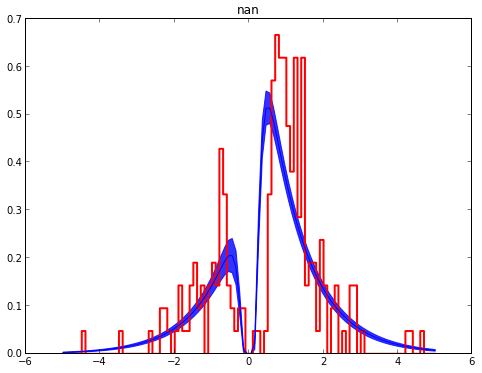
\includegraphics[scale=0.5]{hddm_demo_fig_10.png}

As the above figure shows, the predictive likelihood does not fit the RT data very well. The model predicts far more fast RTs than are actually observed. This is because non-decision time \code{t} is forced to be estimated small enough to account for a few fast RTs.\\

To solve this issue, HDDM includes a mixture model which assumes that outliers come from a uniform distribution. Here, we specify that we expect roughly 5\% outliers in our data. \DUspan{name}{}\DUspan{operator}{}\DUspan{name}{}\DUspan{operator}{}\DUspan{name}{}\DUspan{punctuation}{}\DUspan{name}{}\DUspan{punctuation}{}\DUspan{name}{}\DUspan{operator}{}\DUspan{literal,number,oct}{}\DUspan{punctuation}{}\DUspan{name}{}\DUspan{operator}{}\DUspan{name}{}\DUspan{punctuation}{}\DUspan{literal,number,integer}{}\DUspan{punctuation}{}\DUspan{name}{}\DUspan{operator}{}\DUspan{literal,number,integer}{}\DUspan{punctuation}{}
\begin{Verbatim}[commandchars=\\\{\}]
\PYG{n}{m\PYGZus{}outlier} \PYG{o}{=} \PYG{n}{hddm}\PYG{o}{.}\PYG{n}{HDDM}\PYG{p}{(}\PYG{n}{outlier\PYGZus{}data}\PYG{p}{,} \PYG{n}{p\PYGZus{}outlier}\PYG{o}{=}\PYG{o}{.}\PYG{l+m+mo}{05}\PYG{p}{)}
\PYG{n}{m\PYGZus{}outlier}\PYG{o}{.}\PYG{n}{sample}\PYG{p}{(}\PYG{l+m+mi}{2000}\PYG{p}{,} \PYG{n}{burn}\PYG{o}{=}\PYG{l+m+mi}{20}\PYG{p}{)}
\end{Verbatim}
\DUspan{name}{}\DUspan{operator}{}\DUspan{name}{}\DUspan{punctuation}{}
\begin{Verbatim}[commandchars=\\\{\}]
\PYG{n}{m\PYGZus{}outlier}\PYG{o}{.}\PYG{n}{plot\PYGZus{}posterior\PYGZus{}predictive}\PYG{p}{(}\PYG{p}{)}
\end{Verbatim}

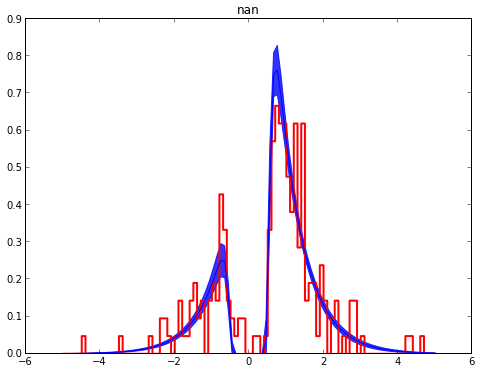
\includegraphics[scale=0.5]{hddm_demo_fig_11.png}

The mixture model provides a much better fit because outlier RTs are having less of an effect because they get assigned to the uniform outlier distribution. Note that it is also possible to estimate the probability of obtaining outliers from the data by setting \code{include=['p\_outlier']} instead of \code{p\_outlier=x} when \code{HDDM} in instantiated.

\section*{Discussion}
We developed an open-source Python toolbox that allows hierarchical Bayesian parameter estimation of the DDM and LBA and is successfully being used in various experimental psychology and neurocognitive research laboratories. The DDM and LBA can be used to infer latent psychological processes underlying decision making given reaction time and choice data. The benefit of the hierarchical Bayesian approach is two-fold: (i) improved accuracy of individual subject parameter estimation by explicitly modeling subject similarity in a hierarchical fashion; and (ii) full Bayesian posterior inference that obsoletes frequentist statistics and confidence intervals. Despite prior methodological advancements in this area \citep{VandekerckhoveTuerlinckxLee11}, a reliable software package implementing this method was previously not available. A simple yet powerful model description mechanism allows the creation of arbitrarily complex models where separate parameters can be estimated for different conditions. Additional features like posterior-predictive-checks allow for model validation and comparison. Finally, to facilitate cross-domain application of this toolbox in the cognitive neurosciences, it is simple to estimate trial-by-trial influences of e.g. brain-measures on individual model parameters.

Using data from our lab on a reward-based learning and decision making task \citep{CavanaghWieckiCohenEtAl11} we demonstrate how this toolbox can successfully be used to estimate differences in information processing based solely on RT and choice data. We then extended this analysis to estimate within-subject effects. By using the \code{HDDMRegression} model we are able to not only quantify latent decision making processes in individuals but also how these latent processes relate to brain measures (here theta power as measured by EEG had a positive effect on threshold) on a trial-by-trial basis. Critically, changing brain state via DBS revealed that the effect of theta power on threshold was reversed. As these trial-by-trial effects are often quite noisy, our hierarchical Bayesian approach facilitated the detection of this effect, due to shared statistical structure among subjects in determining model parameters. This analysis is more informative than a straight behavioral relationship between brain activity and RT or accuracy alone. While we used EEG to measure brain activity this method should be easily extendable towards other techniques like fMRI. While trial-by-trial BOLD responses from an event-related study design are often very noisy we obtained promising results in our lab with this approach.

In conclusion, \code{HDDM} is a novel tool that allows researchers to study the neurocognitive implementations of psychological decision making processes. The hierarchical modeling provides power to detect even small correlations between brain activity and decision making processes. Bayesian estimation supports the recent paradigm shift away from frequentist statistics for hypothesis testing \citep{Lindley65,Kruschke10,LeeWagenmakers13}.

\section*{Acknowledgements}
The authors are thankful to Guido Biele and Øystein Sandvik for useful feedback and code contributions. This work was supported by NIMH Grant RO1 MH080066-01 and NSF Grant \#1125788.

\bibliographystyle{plainnat}
\bibliography{hddm}

\renewcommand{\indexname}{Index}
\printindex
\end{document}
